\chapter{Controller design}%
\label{ch:controller_design}

\section{Current controller}
\label{sec:controller_design_current_controller}

To help fascilitate the design of the position and torque controllers, we will first design a controller for the armature current $I_a$ with the armature voltage $E_a$. This will allow us to treat the armature current as a control input in the position control design, simplifying the dynamics significantly. As the dynamics of the armature current is so fast, the controller has to be as cheap as possible to compute. Hence, it will be designed as a simple proportional (P) controller, but with a feedforward (FF) term to account for the back EMF. Let's first consider the electrical dynamics of the motor from \cref{eq:motor_model_electrical_rewrite}:

\begin{equation}
    \label{eq:controller_design_electrical_dynamics}
    L_a \frac{\mathrm{d}I_a}{\mathrm{d}t} + R_a I_a + K_b \frac{\mathrm{d}\theta}{\mathrm{d}t}= E_a.
\end{equation}

Given the time varying reference current $r(t)$, we can design the input voltage $E_a(t)$ as:

\begin{equation}
    \label{eq:controller_design_voltage_input}
    E_a(t) = \underbrace{K_b \frac{\mathrm{d}\theta(t)}{\mathrm{d}t}}_{\text{Feedforward term}} + \;\underbrace{L_a K_p \left(r(t) - I_a(t)\right)}_{\text{P controller}}.
\end{equation}

Substituting \cref{eq:controller_design_voltage_input} into \cref{eq:controller_design_electrical_dynamics}, we get:

\begin{equation}
    \label{eq:controller_design_current_dynamics}
    \frac{\mathrm{d}I_a(t)}{\mathrm{d}t} + R_a I_a(t) = K_p (r(t) - I_a(t)) \triangleq u(t).
\end{equation}

This controller is supposed to be ran in real time on a microcontroller. That way it won't have access to continuous time signals, but rather discrete time signals. Hence, we will need to discretize the controller for stability analysis and tuning. For this analysis we will assume that the dynamics of the motor are slow enough such that the feedforward term can be treated as a constant. This is a reasonable assumption since the feedforward term is based on the angular velocity, which changes relatively slowly compared to the armature current.

\subsection{Discretization of current controller}
Suppose the controller is ran with a update period of $T_s$. Assuming that the input voltage $E_a$ is held constant between sampling times, i.e.,

\begin{equation}
    \label{eq:controller_design_discretized_input}
    u(t)=u[k] = K_p (r[k] - I_a[k]), \quad k T_s \leq t < (k+1)T_s,
\end{equation}

the dynamics in \cref{eq:controller_design_current_dynamics} then becomes:

\begin{equation}
    \label{eq:controller_design_current_interval_dynamics}
    \frac{\mathrm{d}I_a(\tau)}{\mathrm{d}\tau} + R_a I_a(\tau) = u[k], \quad \tau = t - k T_s \in [0, T_s].
\end{equation}

To solve it, let's multiply by the integrating factor $e^{R_a \tau}$, which gives:

\begin{equation}
    \label{eq:controller_design_current_integrating_factor}
    e^{R_a \tau} \left[\frac{\mathrm{d}I_a(\tau)}{\mathrm{d}\tau} + R_a I_a(\tau)\right] = u[k] e^{R_a \tau}.
\end{equation}

Notice how this can be rewritten as:

\begin{equation}
    \label{eq:controller_design_current_integrating_factor_rewrite}
    \frac{\mathrm{d}}{\mathrm{d}\tau} \left(e^{R_a \tau} I_a(\tau)\right) = u[k] e^{R_a \tau}.
\end{equation}

Integrating both sides of \cref{eq:controller_design_current_integrating_factor_rewrite} with respect to $\tau$, over the entire interval from $0$ to $T_s$, we get the discretized dynamics of the current controller:

\begin{equation}
    \label{eq:controller_design_discretized}
    \begin{aligned}
        [e^{R_a \tau} I_a(\tau)]_{\tau = 0}^{\tau = T_s} &= u[k] \int_0^{T_s} e^{R_a \tau} \mathrm{d}\tau,\\
        \implies e^{R_a T_s} \underbrace{I_a(T_s)}_{I_a[k+1]} - \underbrace{I_a(0)}_{I_a[k]} &= u[k] \frac{e^{R_a T_s} - 1}{R_a},\\
        \implies I_a[k+1] &= \underbrace{e^{-R_a T_s}}_{\triangleq a} I_a[k] + u[k] \underbrace{\frac{1 - e^{-R_a T_s}}{R_a}}_{\triangleq b},\\
        \implies I_a[k+1] &= a I_a[k] + b u[k].
    \end{aligned}
\end{equation}

Substituting in $u[k]$ from \cref{eq:controller_design_discretized_input}, we get:

\begin{equation}
    \label{eq:controller_design_discretized_reference}
    \begin{aligned}
        I_a[k+1] &= a I_a[k] + b K_p (r[k] - I_a[k]),\\
        \implies I_a[k+1] &= \left(a - b K_p\right) I_a[k] + b K_p r[k].
    \end{aligned}
\end{equation}



\subsection{Stability analysis and tuning of controller}

To guarantee stability of the current controller, we can look at the z-transform of the system. Taking the z-transform of \cref{eq:controller_design_discretized_reference}, disregarding any initial conditions, we get:

\begin{equation}
    \label{eq:controller_design_current_dynamics_z_transform}
    \begin{aligned}
        \left[z - (a - b K_p)\right] I_a(z) &= b K_p r(z),\\
        \implies \frac{I_a(z)}{r(z)} &= \frac{b K_p}{z - (a - b K_p)}.
    \end{aligned}
\end{equation}

Clearly, \cref{eq:controller_design_current_dynamics_z_transform} has a pole at $z = a - b K_p$. As discussed in [\textbf{ADD REFERENCE TO THEORY: DISCRETIZED SYSTEMS}], for the system to be stable, we need the pole to be inside the unit circle. In other words, we need:

\begin{equation}
    \label{eq:controller_design_current_stability_condition}
    \begin{aligned}
        |a - b K_p| &< 1 \implies \left|e^{-R_a T_s} - K_p \frac{1 - e^{-R_a T_s}}{R_a}\right| < 1,\\
        \implies K_p &< R_a \frac{1 + e^{-R_a T_s}}{1 - e^{-R_a T_s}} \triangleq K_{p,\text{max}}(T_s).
    \end{aligned}
\end{equation}

One downside to using a P controller is that there will be a steady-state error. To eliminate this, we can artifically give the controller a higher reference current. To do this we will need to know the steady-state value of the current for a given reference. Assuming we apply a step reference of $r[k] = r_0$ for all $k \geq 0$. Provided we choose a $K_p$ that satisfies \cref{eq:controller_design_current_stability_condition}, the recursion will converge, and as we let $t \to \infty \implies k \to \infty$, \cref{eq:controller_design_discretized_reference} becomes:

\begin{equation}
    \label{eq:controller_design_current_steady_state}
    \begin{aligned}
        I_a[\infty] &= (a - b K_p) I_a[\infty] + b K_p r_0,\\
        \implies I_a[\infty] &= r_0 \frac{b K_p}{1 - a + b K_p} = r_0 \frac{\frac{1 - a}{R_a} K_p}{1 - a + \frac{1 - a}{R_a} K_p} = r_0 \frac{K_p}{R_a + K_p}.
    \end{aligned}
\end{equation}

Hence to eliminate the steady-state error, we can choose the reference to be:
\begin{equation}
    \label{eq:controller_design_current_reference_tuning}
    r_1 = \frac{R_a + K_p}{K_p} r_0 \implies I_a[\infty] = r_1 \frac{K_p}{R_a + K_p} = r_0.
\end{equation}

\subsection{Simulation of current controller}

To evaluate the controller, we will simulate it applied to the motor model developed in \cref{sec:brushed_dc_motor_model}. Using $K_p=\frac{1}{2}K_{p,\text{max}}(T_s)$, where the reference current is a step input of $3$ A, and scaled with regards to \cref{eq:controller_design_current_reference_tuning}. Additionally there is a saturation put on $E_a=\pm\SI{12}{\volt}$. \cref{fig:controller_design_current_controller_simulation_P_vs_PFF_speed} and \cref{fig:controller_design_current_controller_simulation_P_vs_PFF_no_speed} shows a simulation of the P+FF controller aswell as just the P controller, with $T_s = \SI{0.2}{\milli\second}$, where the motor is initially spinning at $\omega_0 = \SI{5}{\radian\per\second}$ and $\omega_0 = \SI{0}{\radian\per\second}$, respectively. \cref{fig:controller_design_current_controller_simulation_noise_0.2ms} and \cref{fig:controller_design_current_controller_simulation_noise_1ms} shows the simulation of the P+FF controller with and without noise to the measurement of $I_a$, with $T_s = \SI{0.2}{\milli\second}$ and $T_s = \SI{1.0}{\milli\second}$, respectively. The noise is a zero-mean Gaussian noise with a standard deviation of $\sigma_{\jnt{I_a}} = \SI{50}{\milli\ampere}$, which is higher than is expected for the system, but it will help us evaluate the robustness of the controller.

\begin{figure}[htbp]
    \centering
    \subcaptionbox{P+FF controller.\label{fig:controller_design_current_controller_simulation_pff_with_speed}}{%
        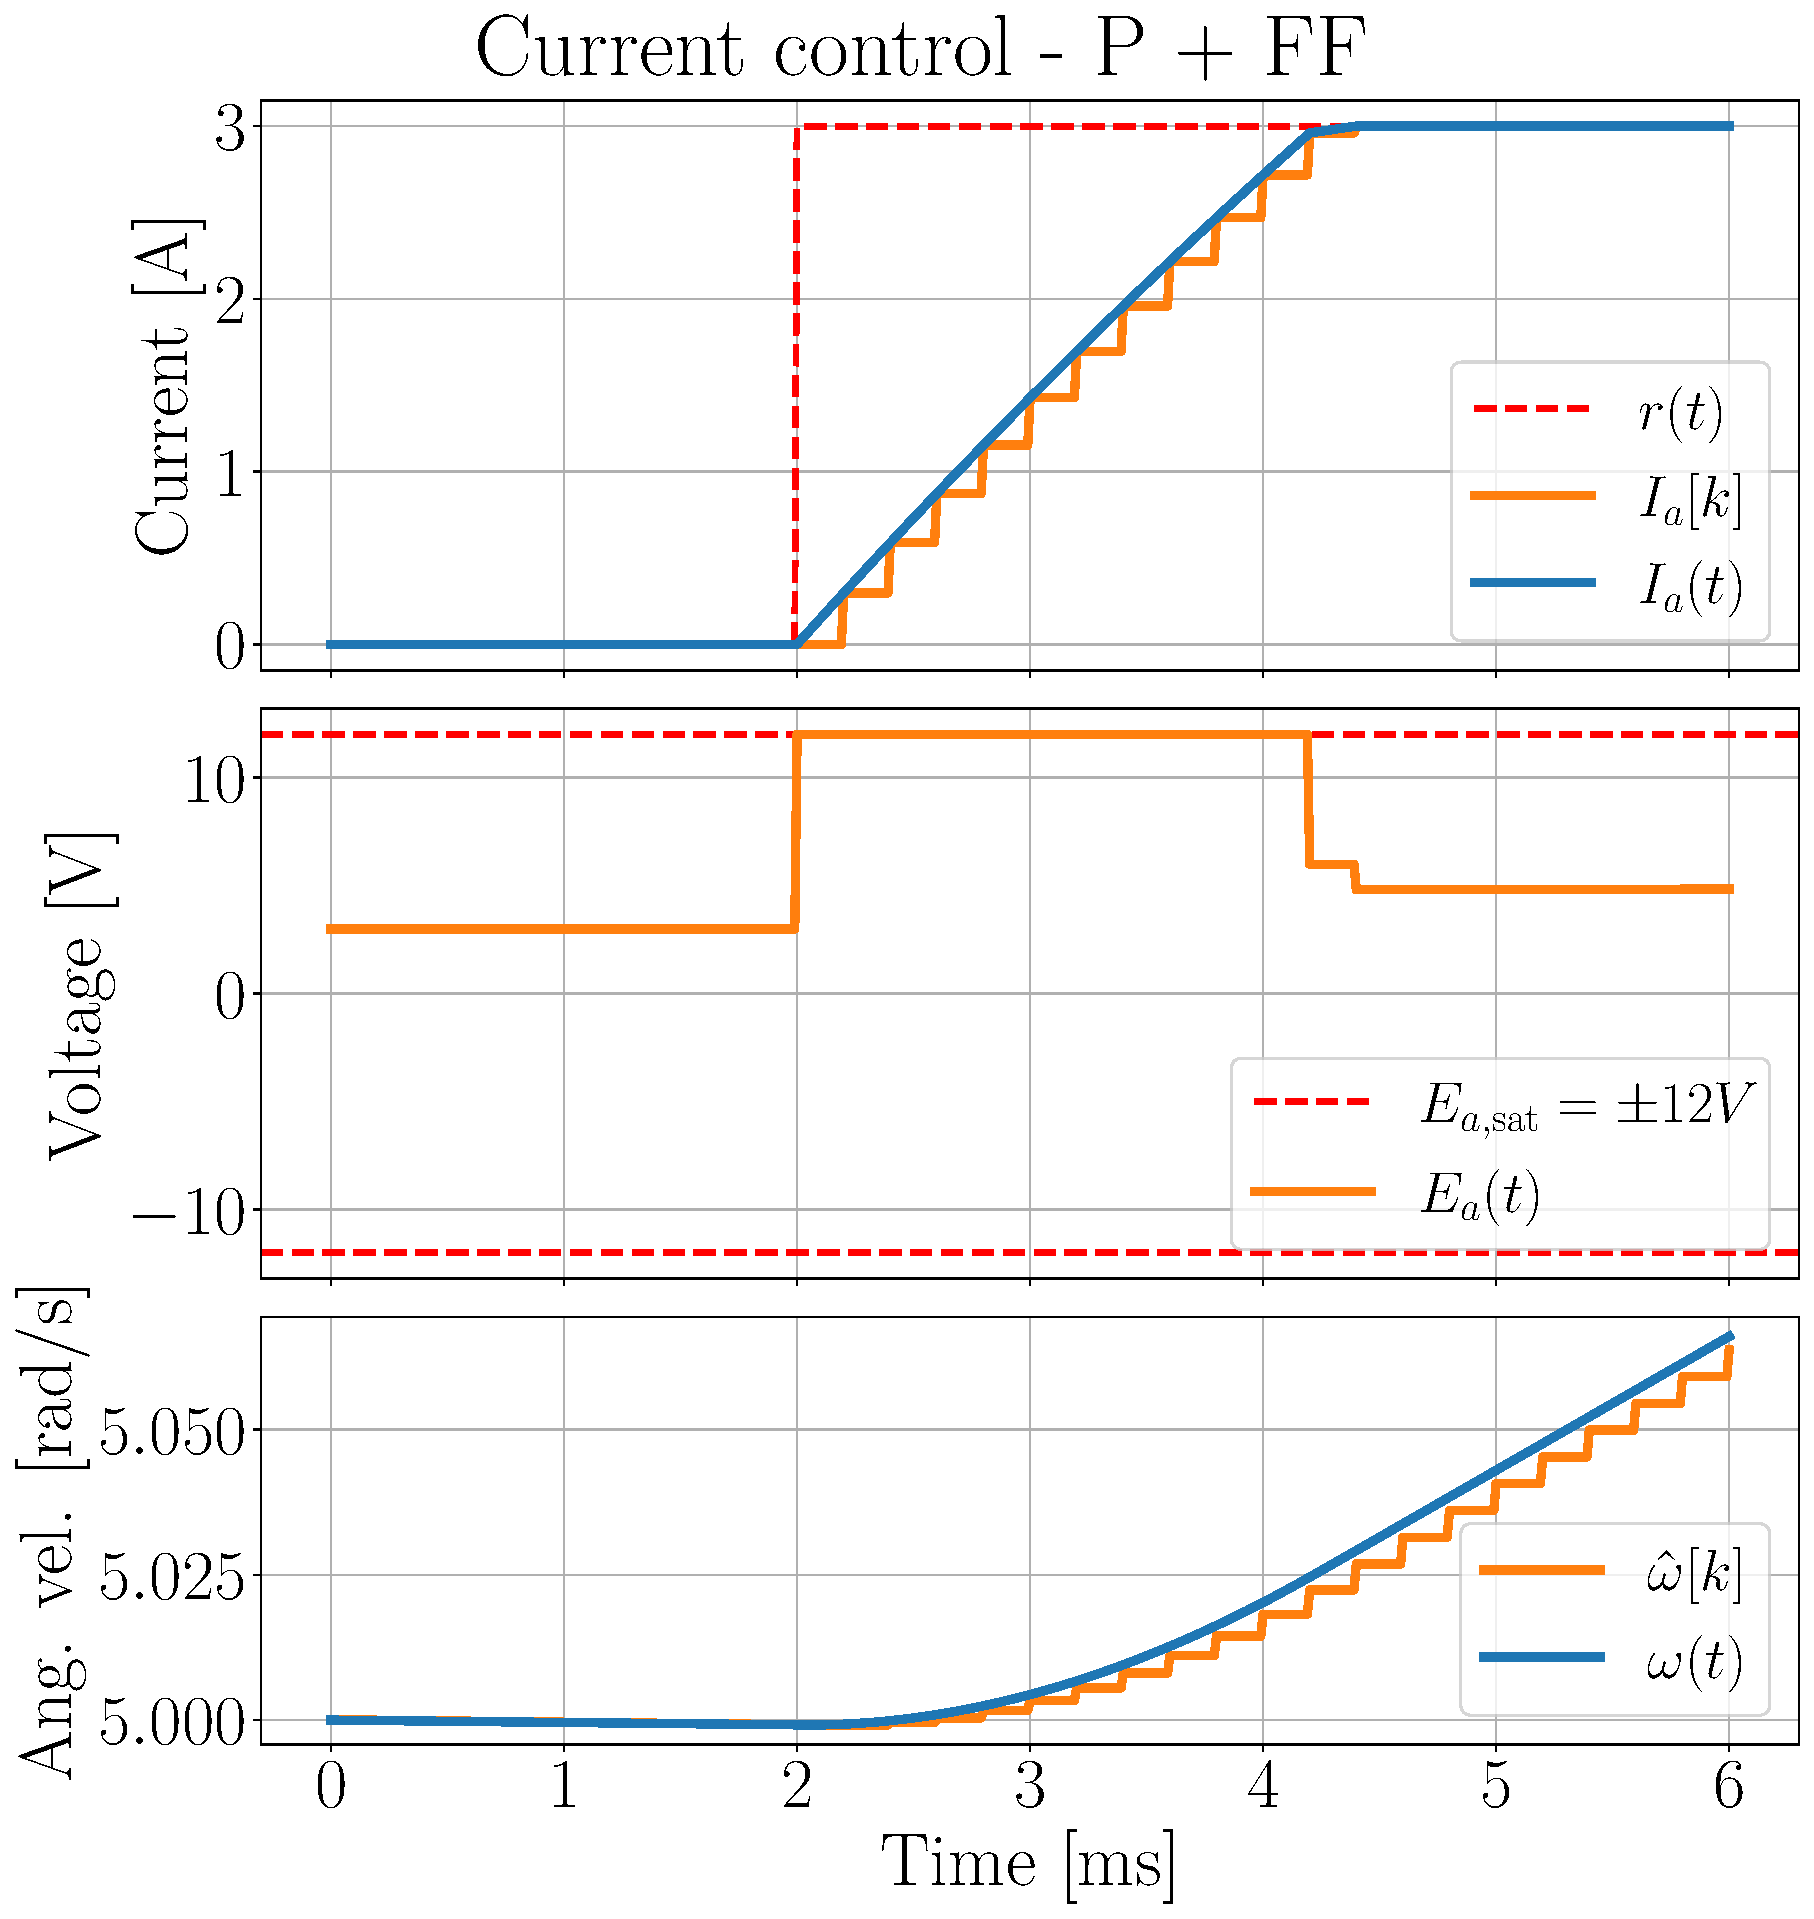
\includegraphics[width=0.49\textwidth]{../Figures/Controller_design/motor_current_control_feed_forward_P_FF_Ts_0.2ms_with_speed.pdf}}
    \hfill
    \subcaptionbox{P controller.\label{fig:controller_design_current_controller_simulation_p_with_speed}}{%
        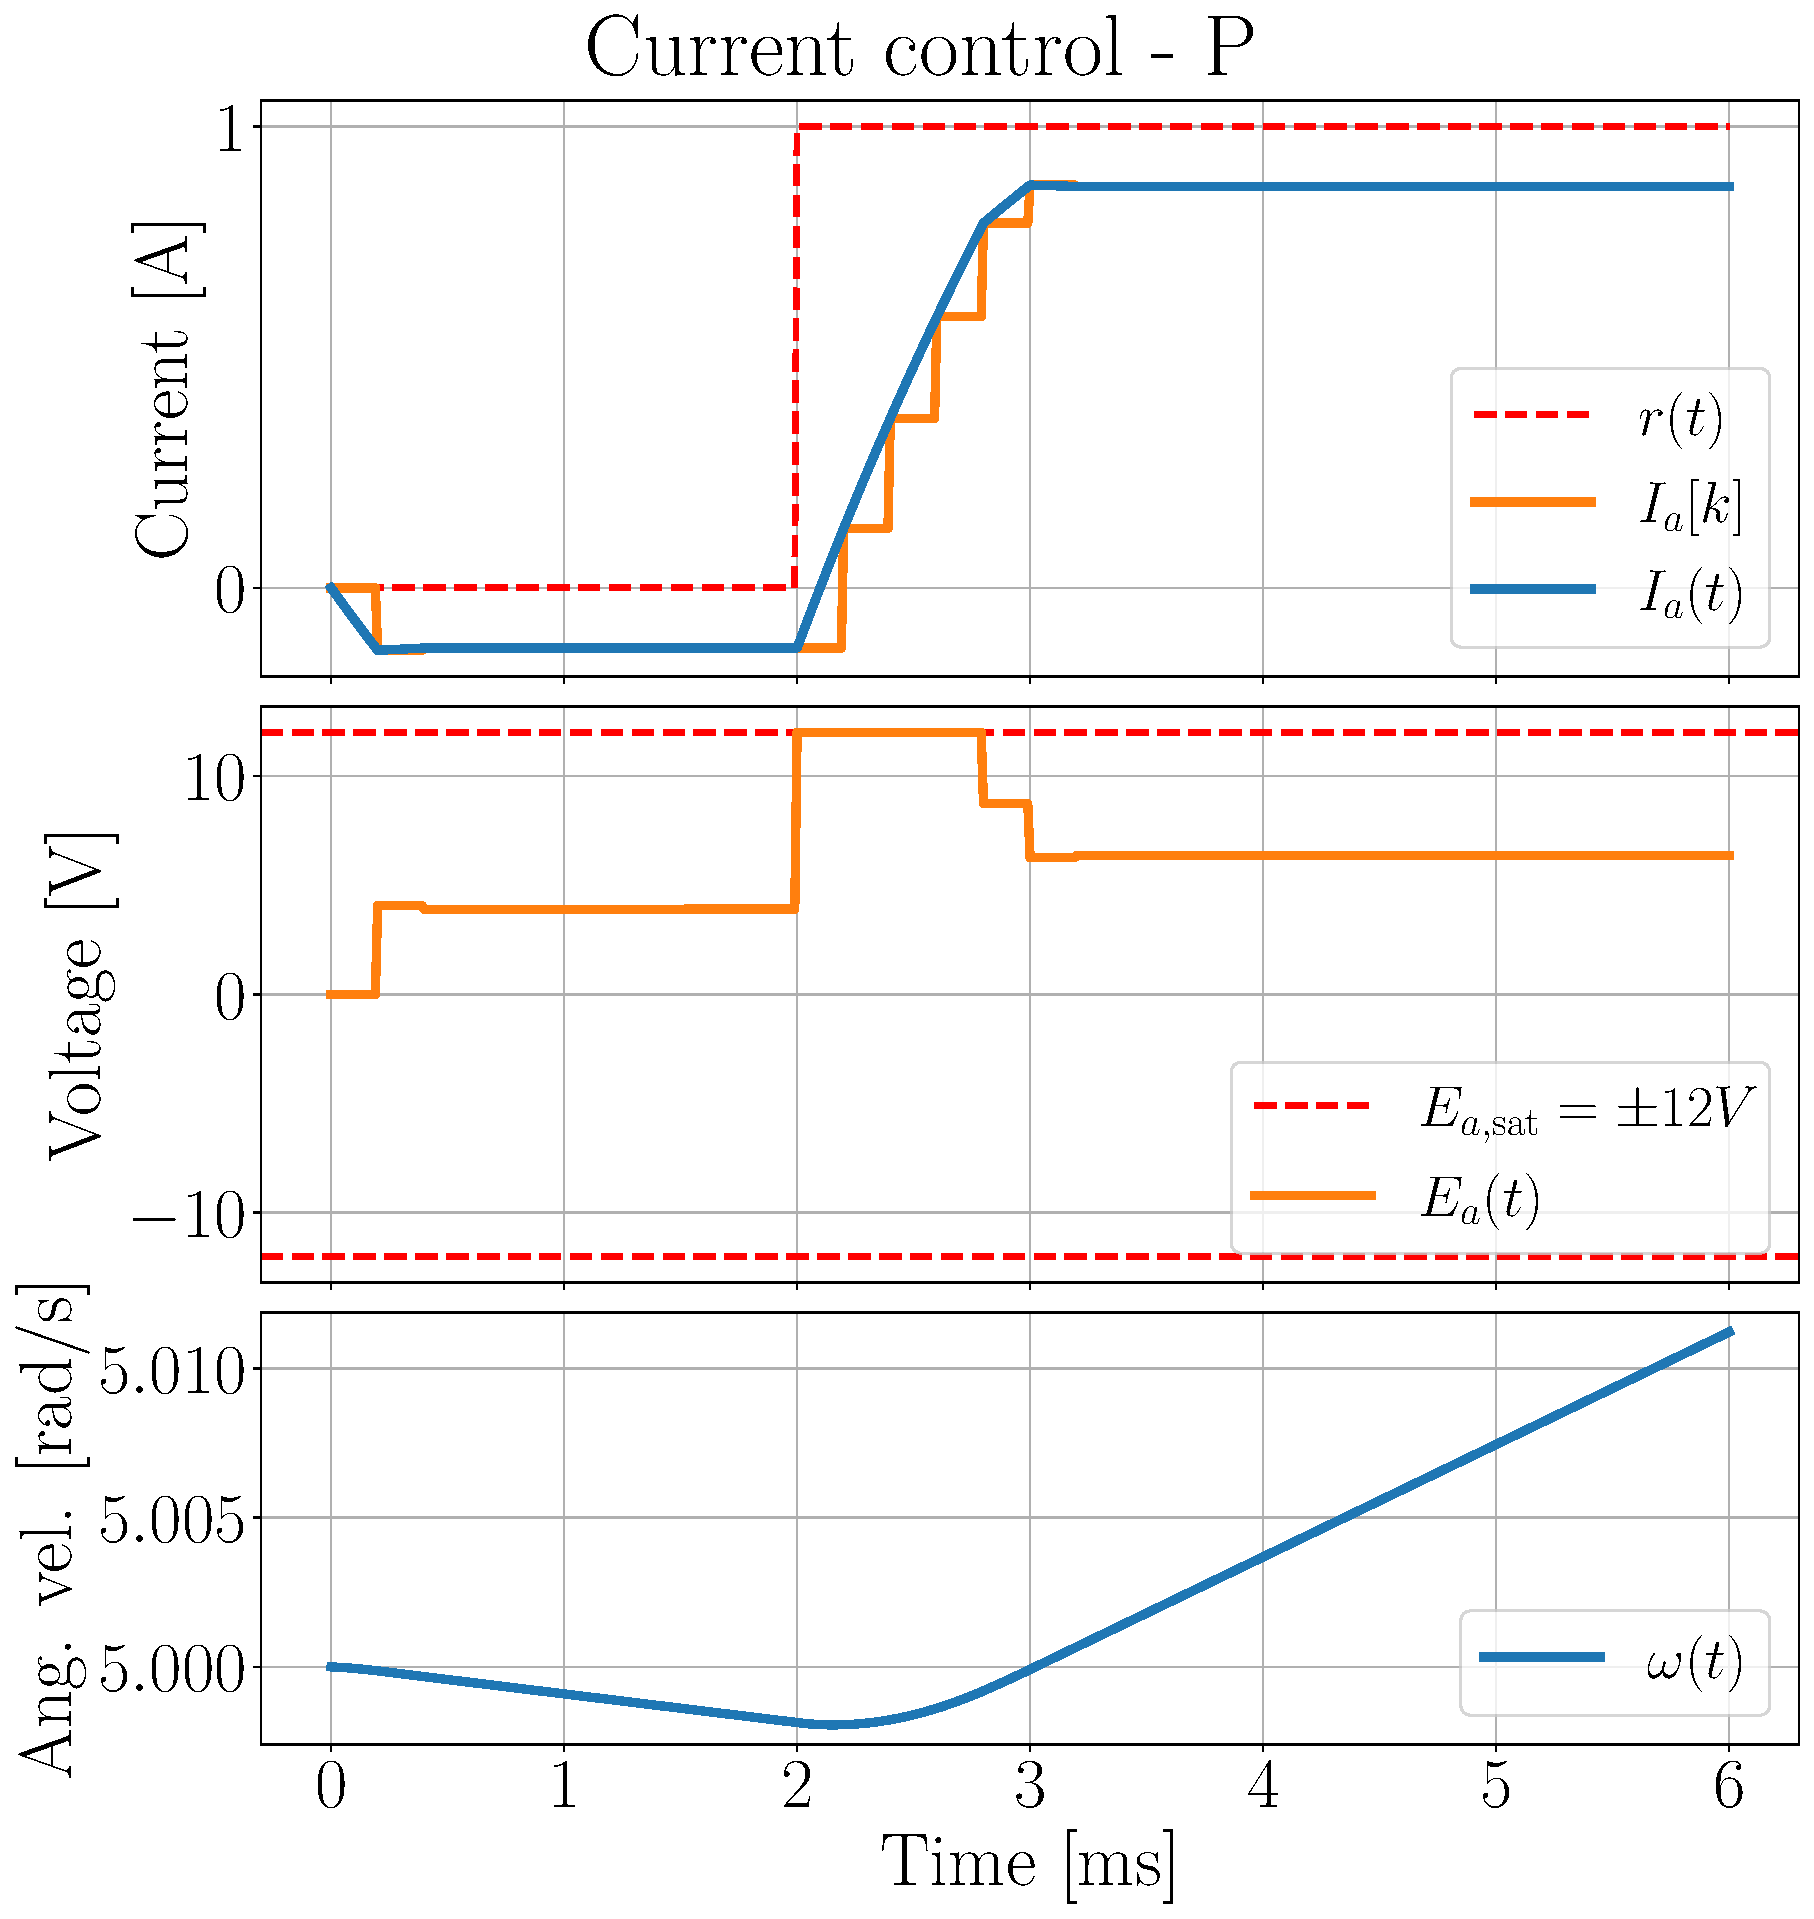
\includegraphics[width=0.49\textwidth]{../Figures/Controller_design/motor_current_control_feed_forward_P_Ts_0.2ms_with_speed.pdf}}
    \caption{P+FF and P controllers with $T_s = \SI{0.2}{\milli\second}$ and $\omega_0 = \SI{5}{\radian\per\second}$.}
    \label{fig:controller_design_current_controller_simulation_P_vs_PFF_speed}
\end{figure}

\begin{figure}[htbp]
    \centering
    \subcaptionbox{P+FF controller.\label{fig:controller_design_current_controller_simulation_pff_no_speed}}{%
        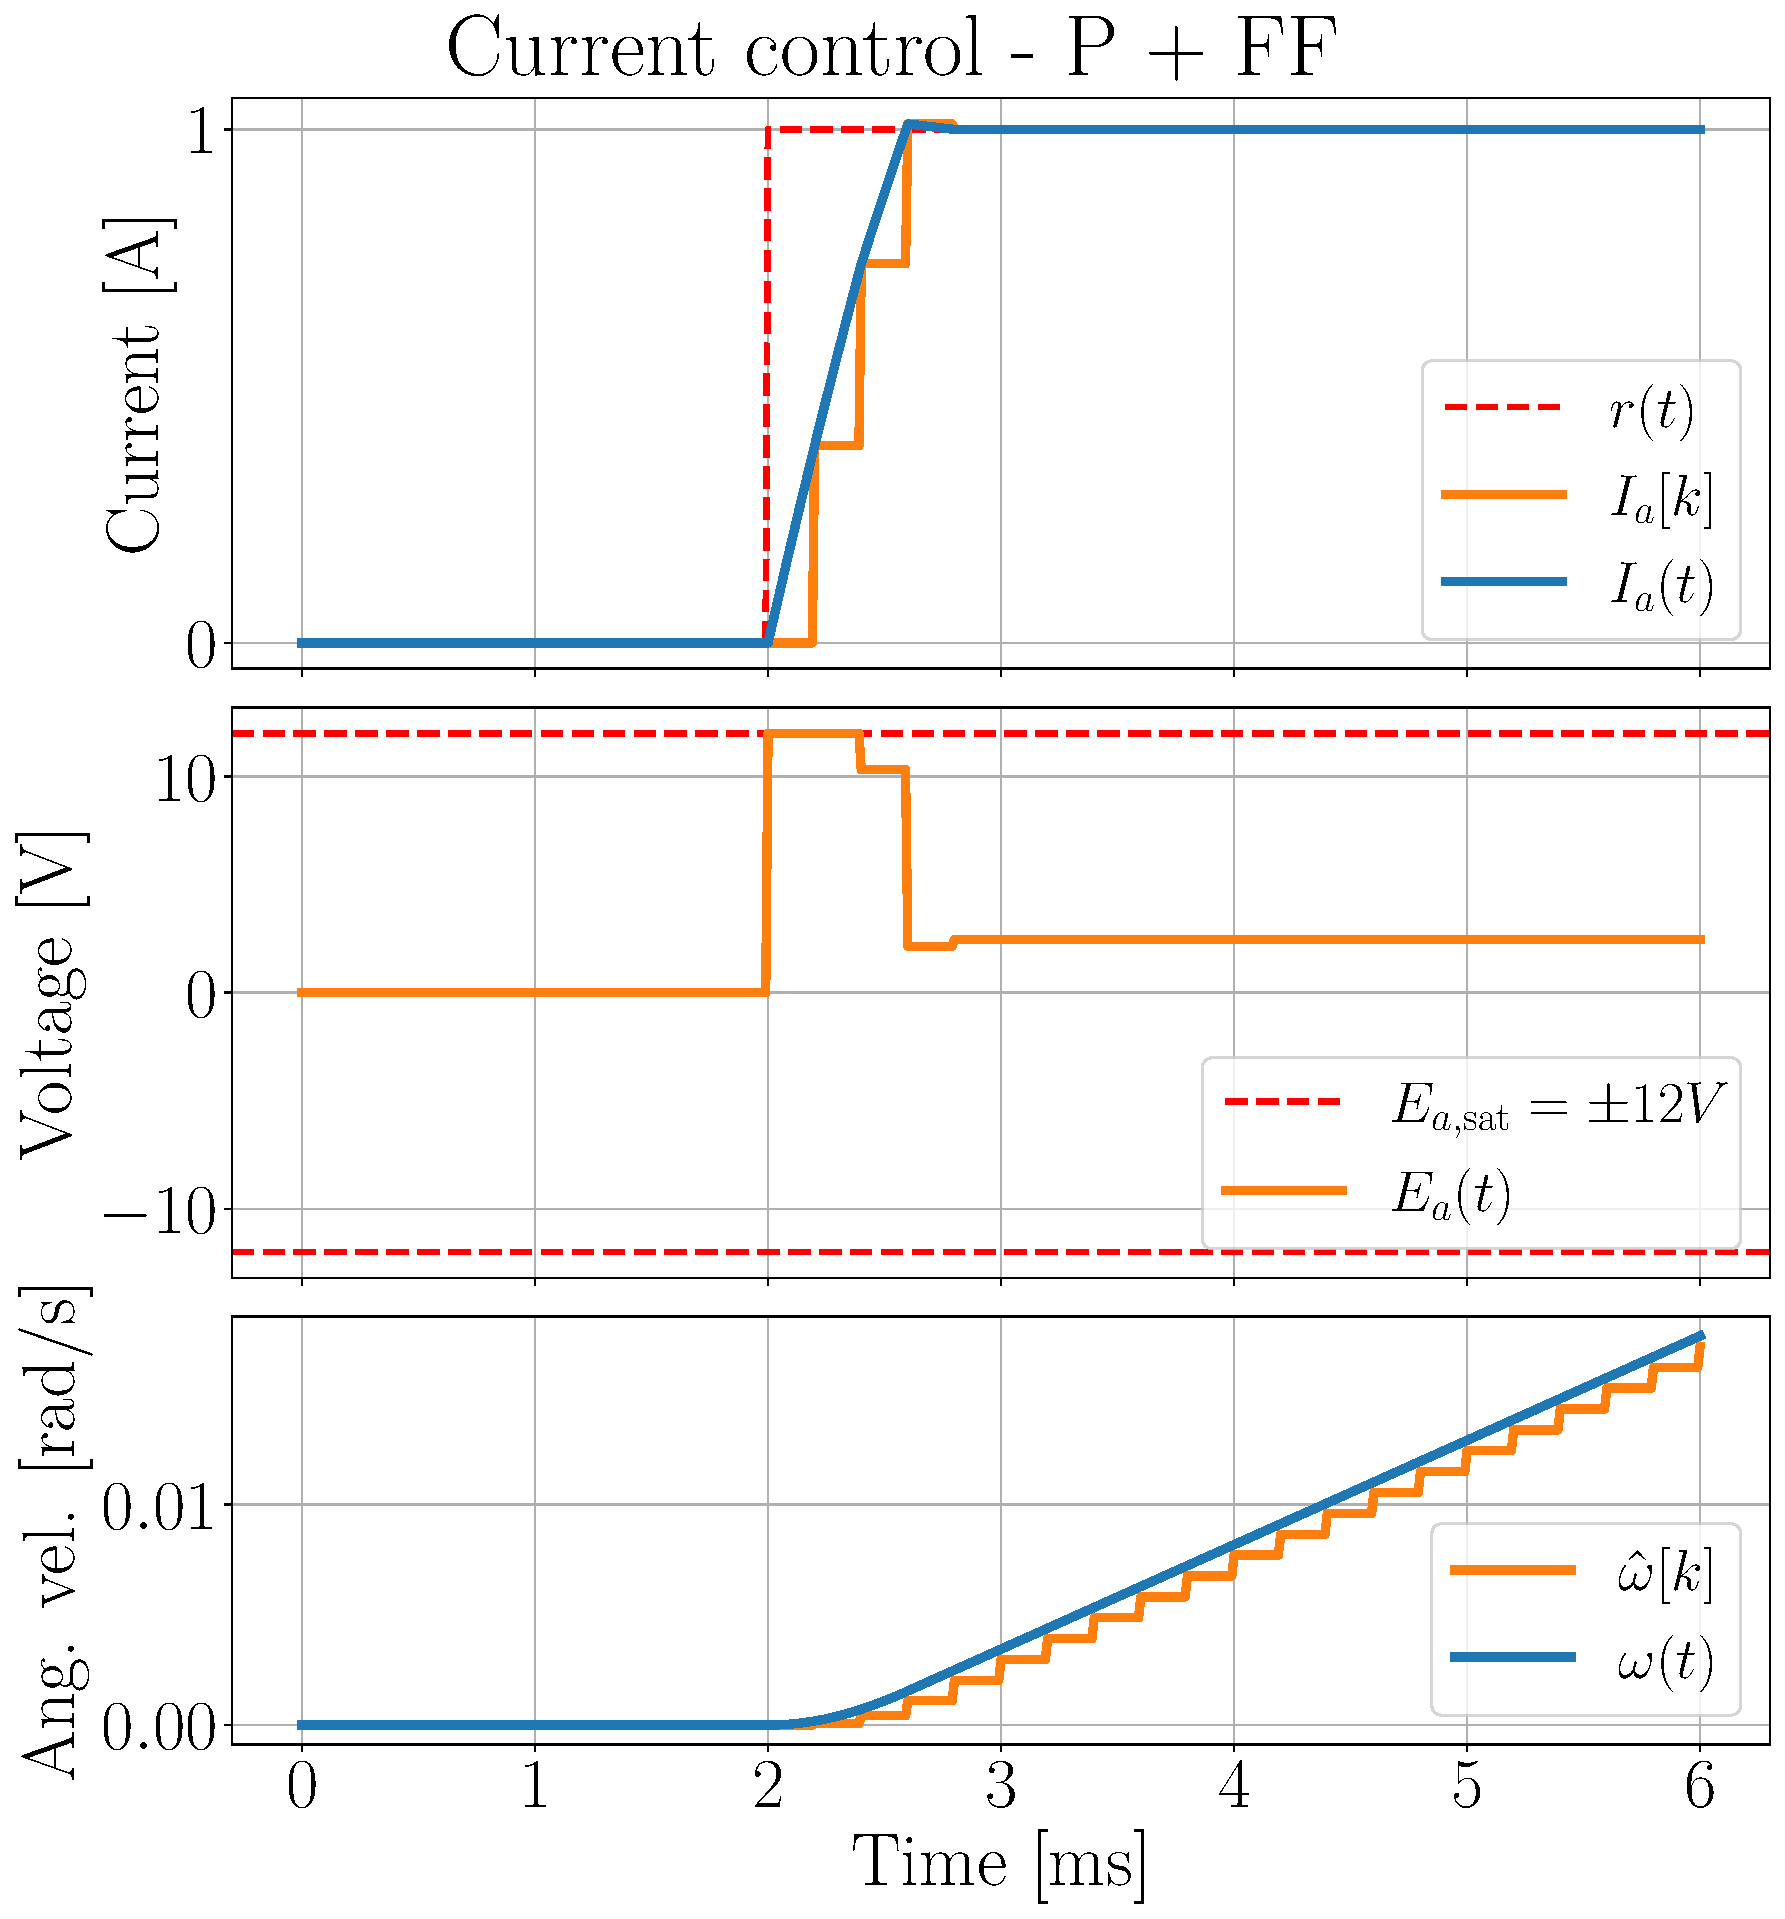
\includegraphics[width=0.49\textwidth]{../Figures/Controller_design/motor_current_control_feed_forward_P_FF_Ts_0.2ms.pdf}}
    \hfill
    \subcaptionbox{P controller.\label{fig:controller_design_current_controller_simulation_p_no_speed}}{%
        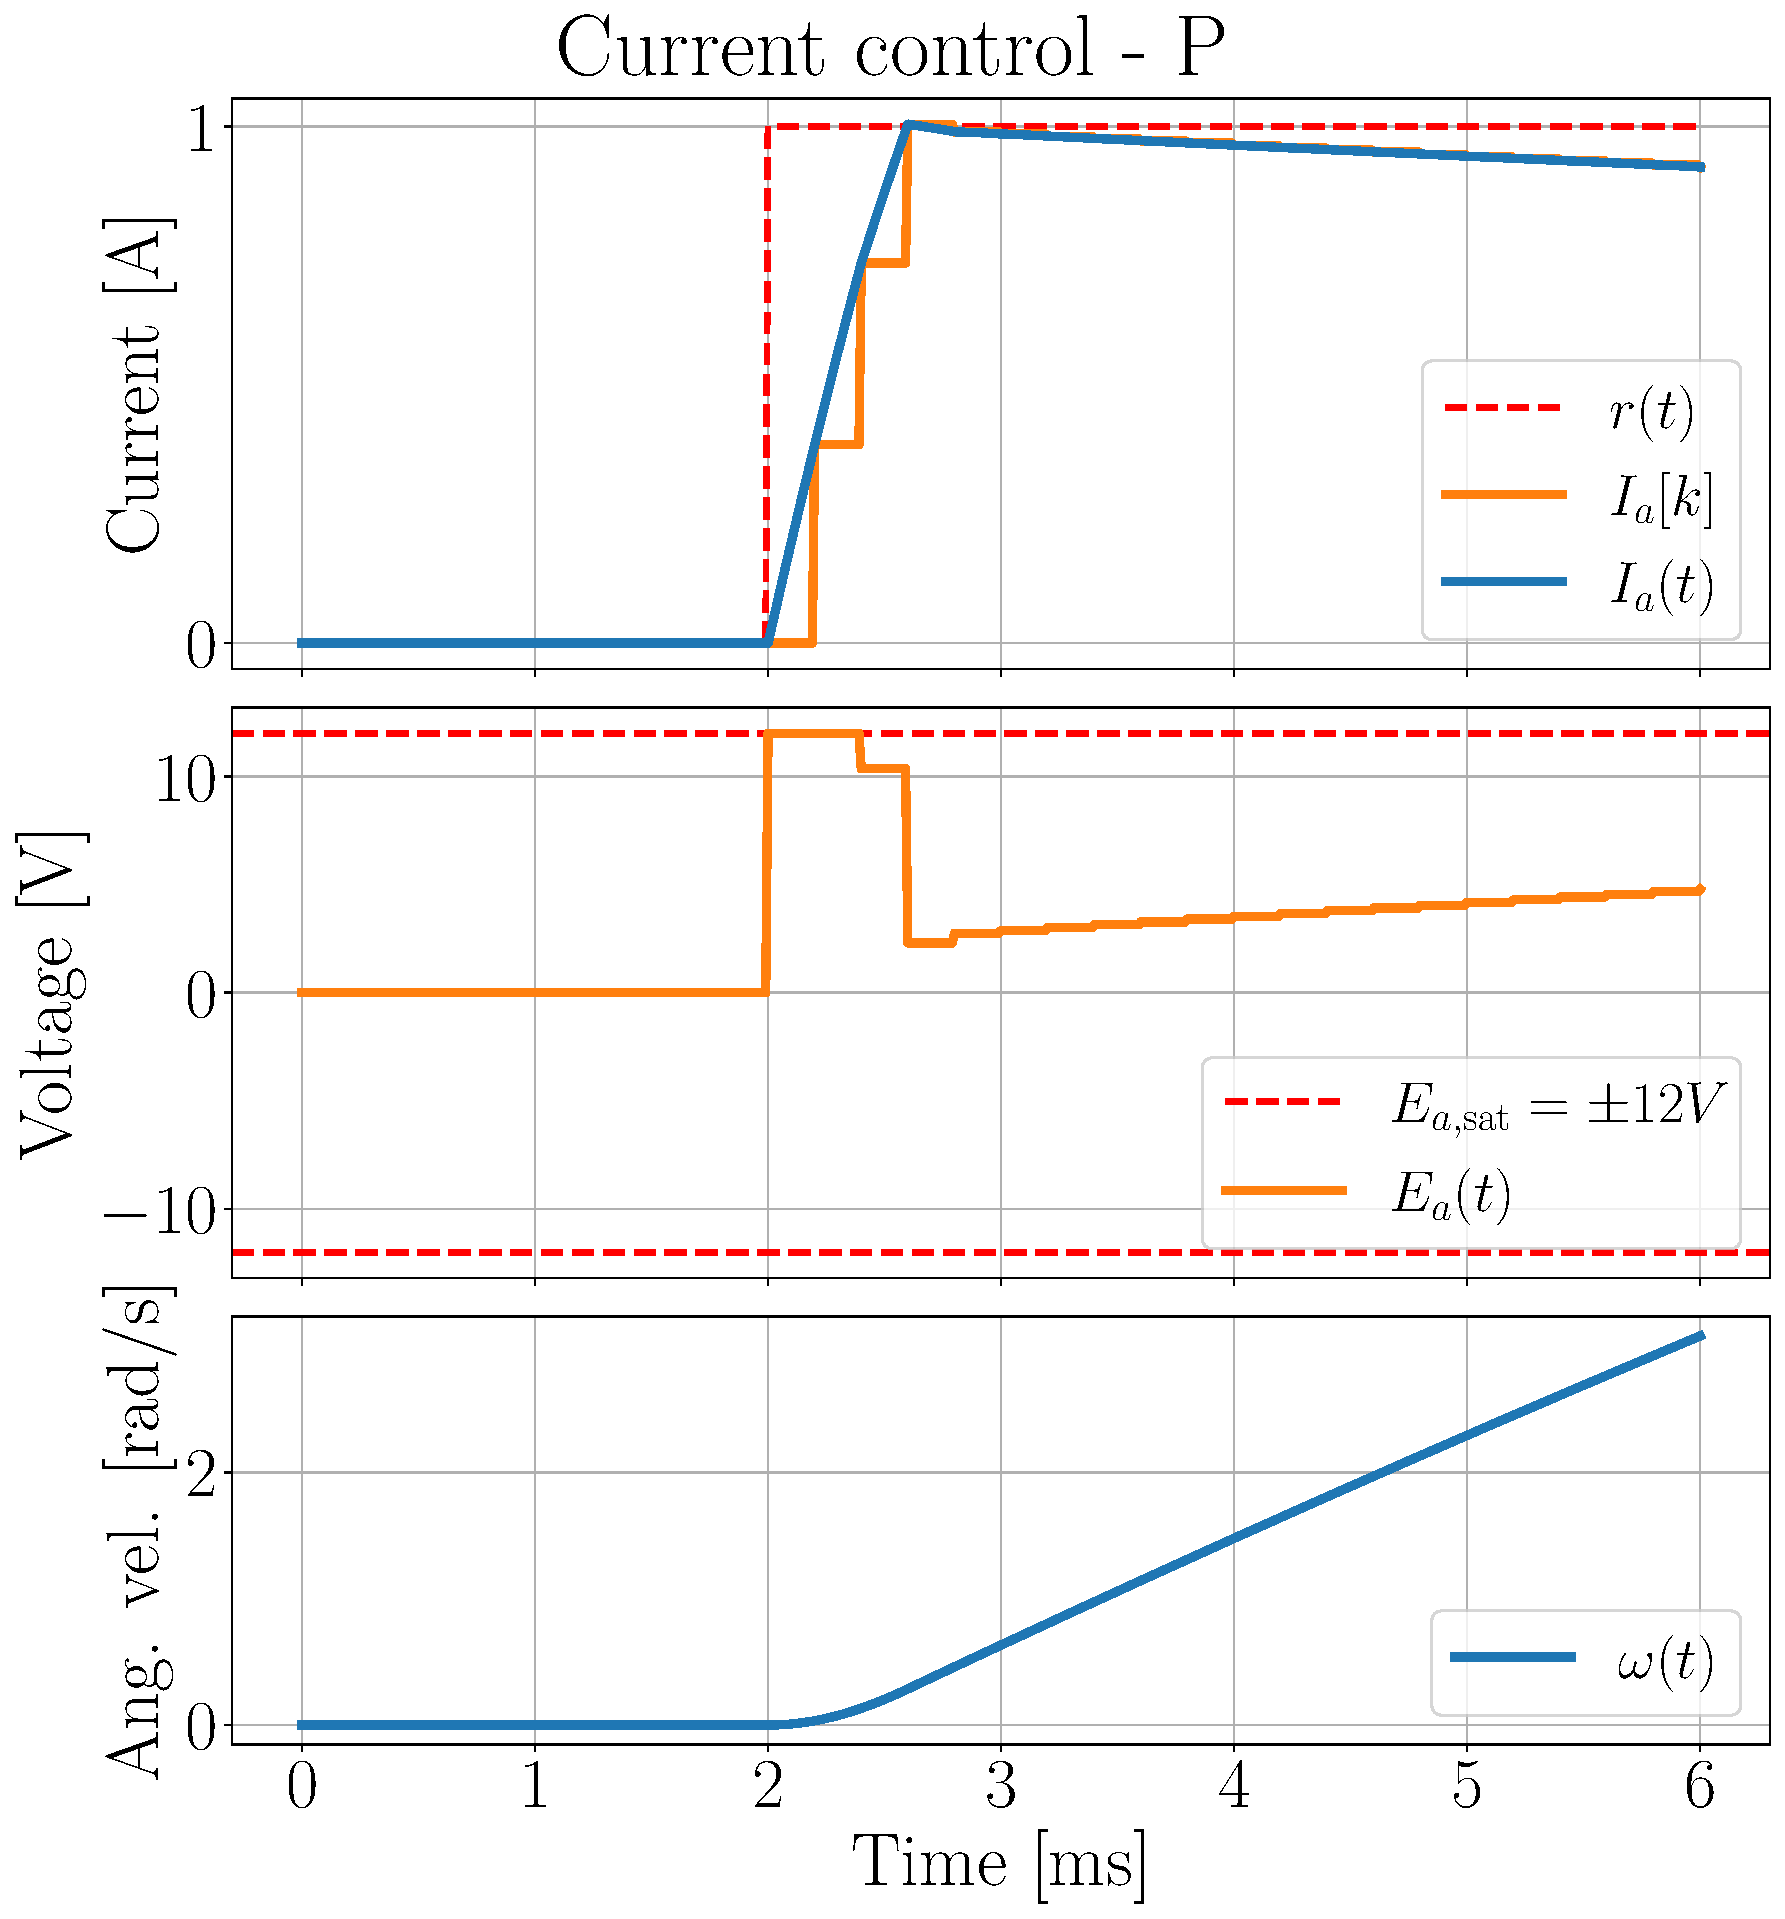
\includegraphics[width=0.49\textwidth]{../Figures/Controller_design/motor_current_control_feed_forward_P_Ts_0.2ms.pdf}}
    \caption{P+FF and P controllers with $T_s = \SI{0.2}{\milli\second}$ and $\omega_0 = \SI{0}{\radian\per\second}$.}
    \label{fig:controller_design_current_controller_simulation_P_vs_PFF_no_speed}
\end{figure}

\begin{figure}[htbp]
    \centering
    \subcaptionbox{Without noise.\label{fig:controller_design_current_controller_simulation_without_noise_0.2ms}}{%
        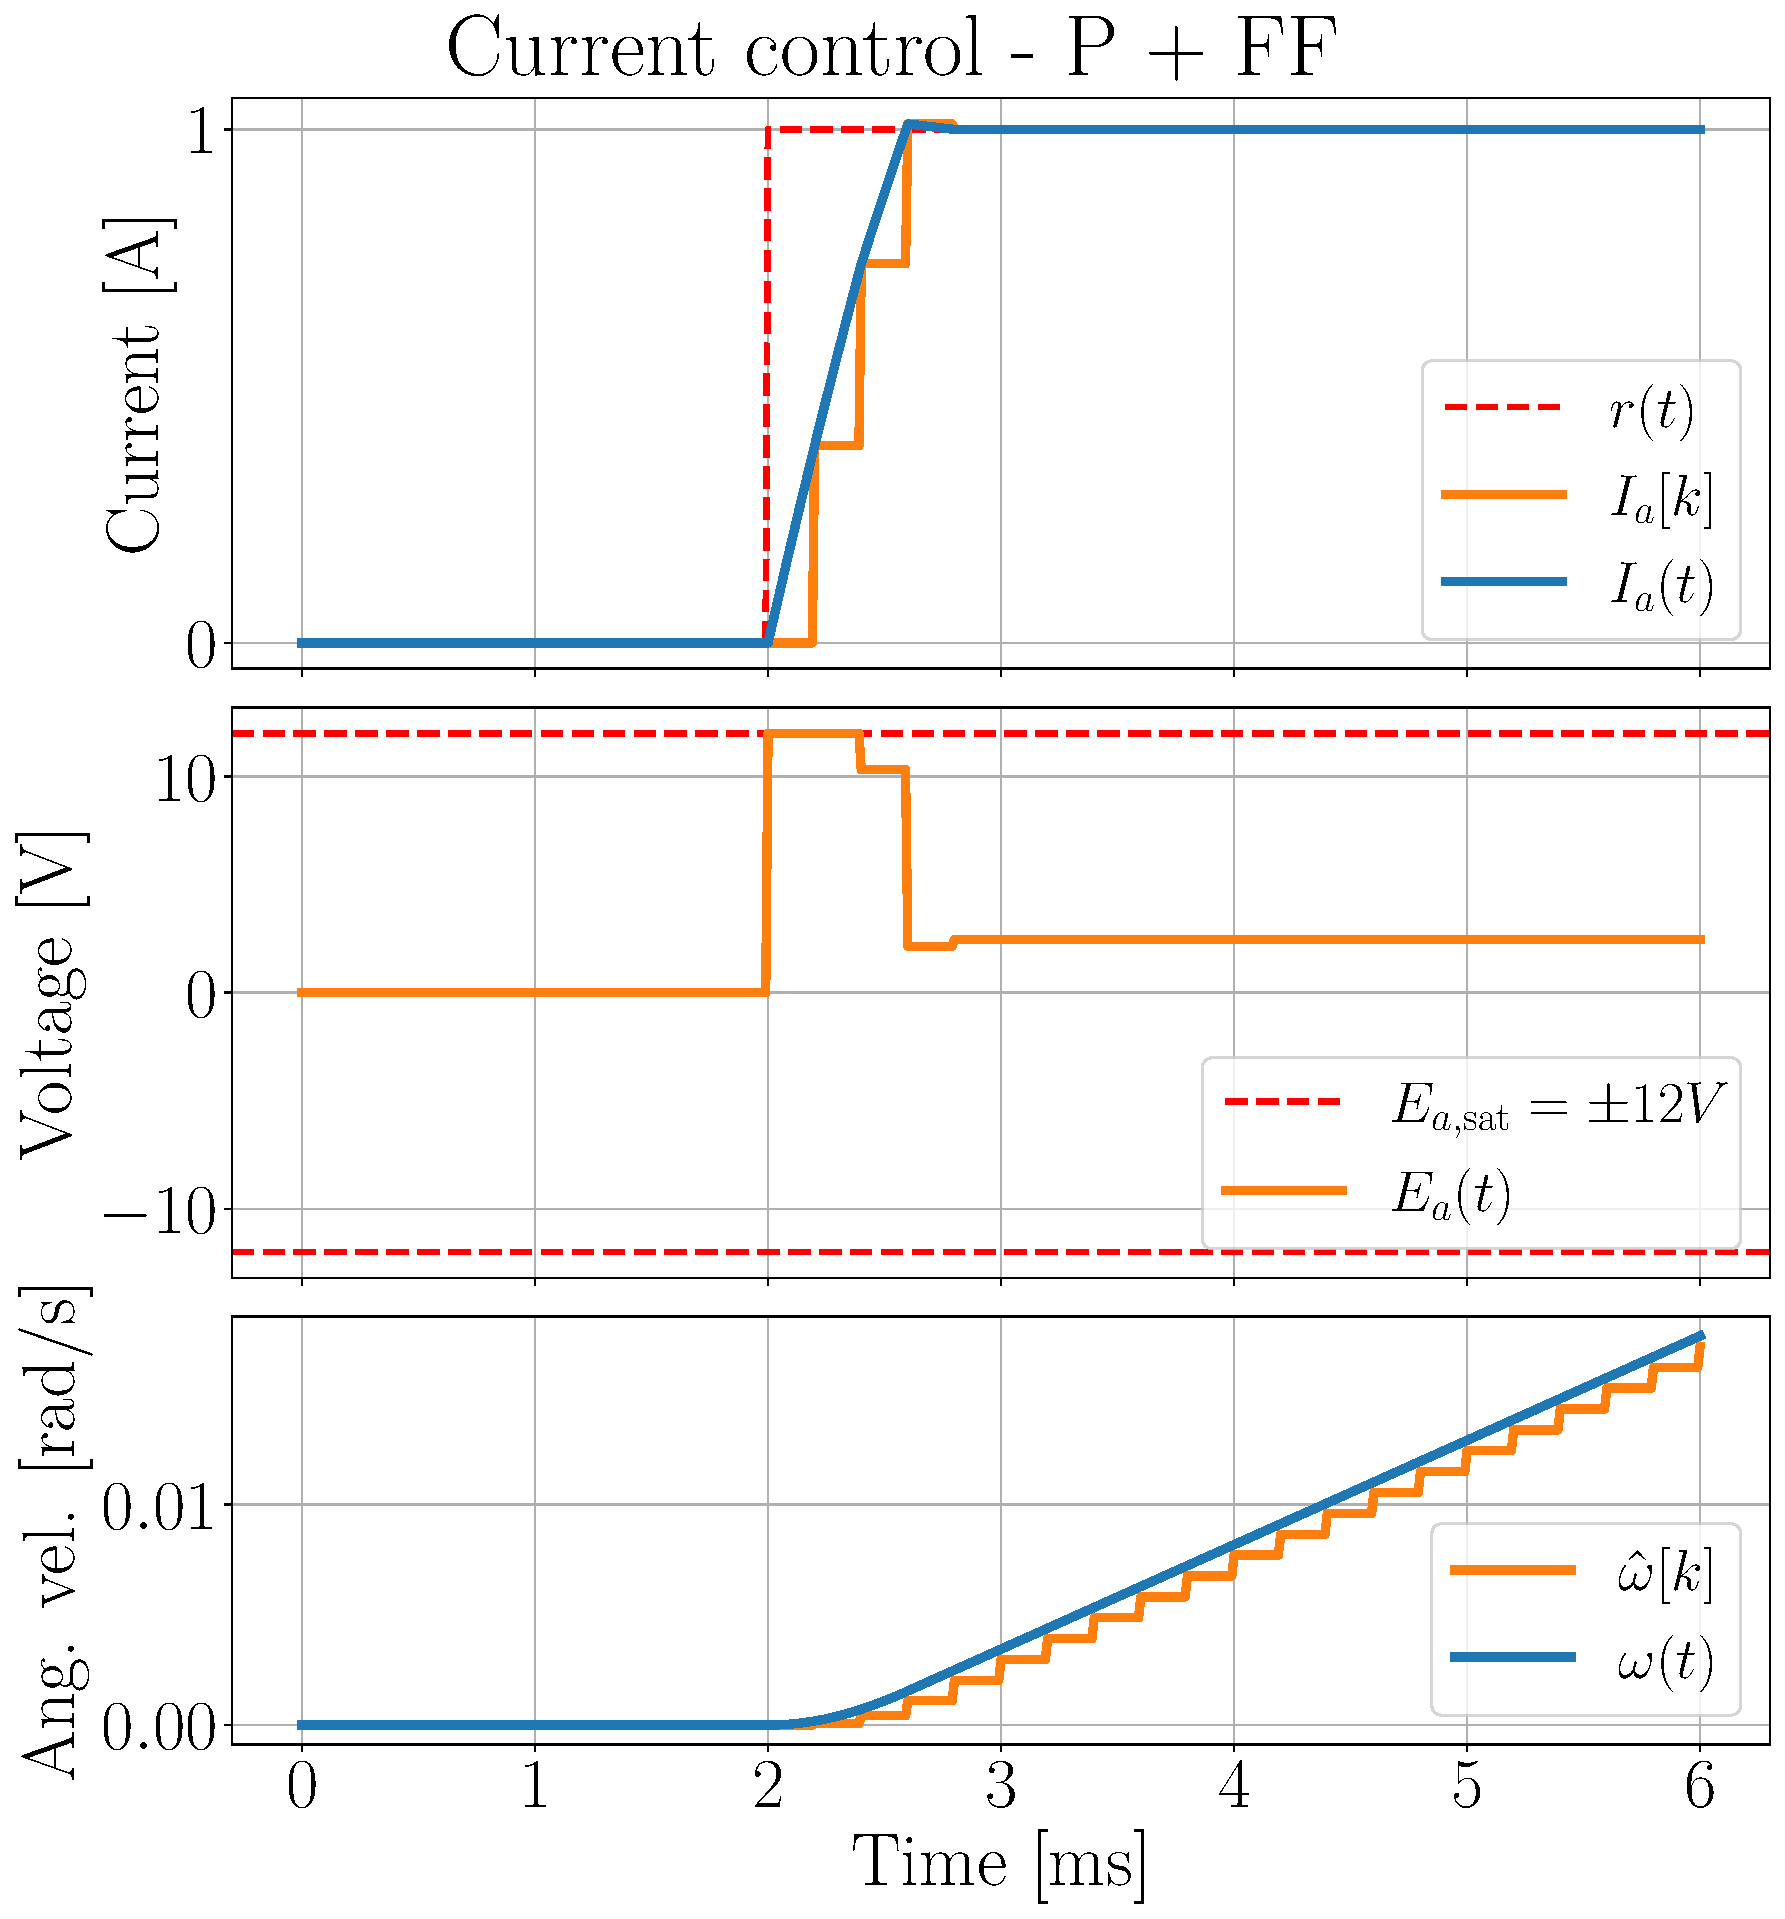
\includegraphics[width=0.49\textwidth]{../Figures/Controller_design/motor_current_control_feed_forward_P_FF_Ts_0.2ms.pdf}}
    \hfill
    \subcaptionbox{With noise.\label{fig:controller_design_current_controller_simulation_with_noise_0.2ms}}{%
        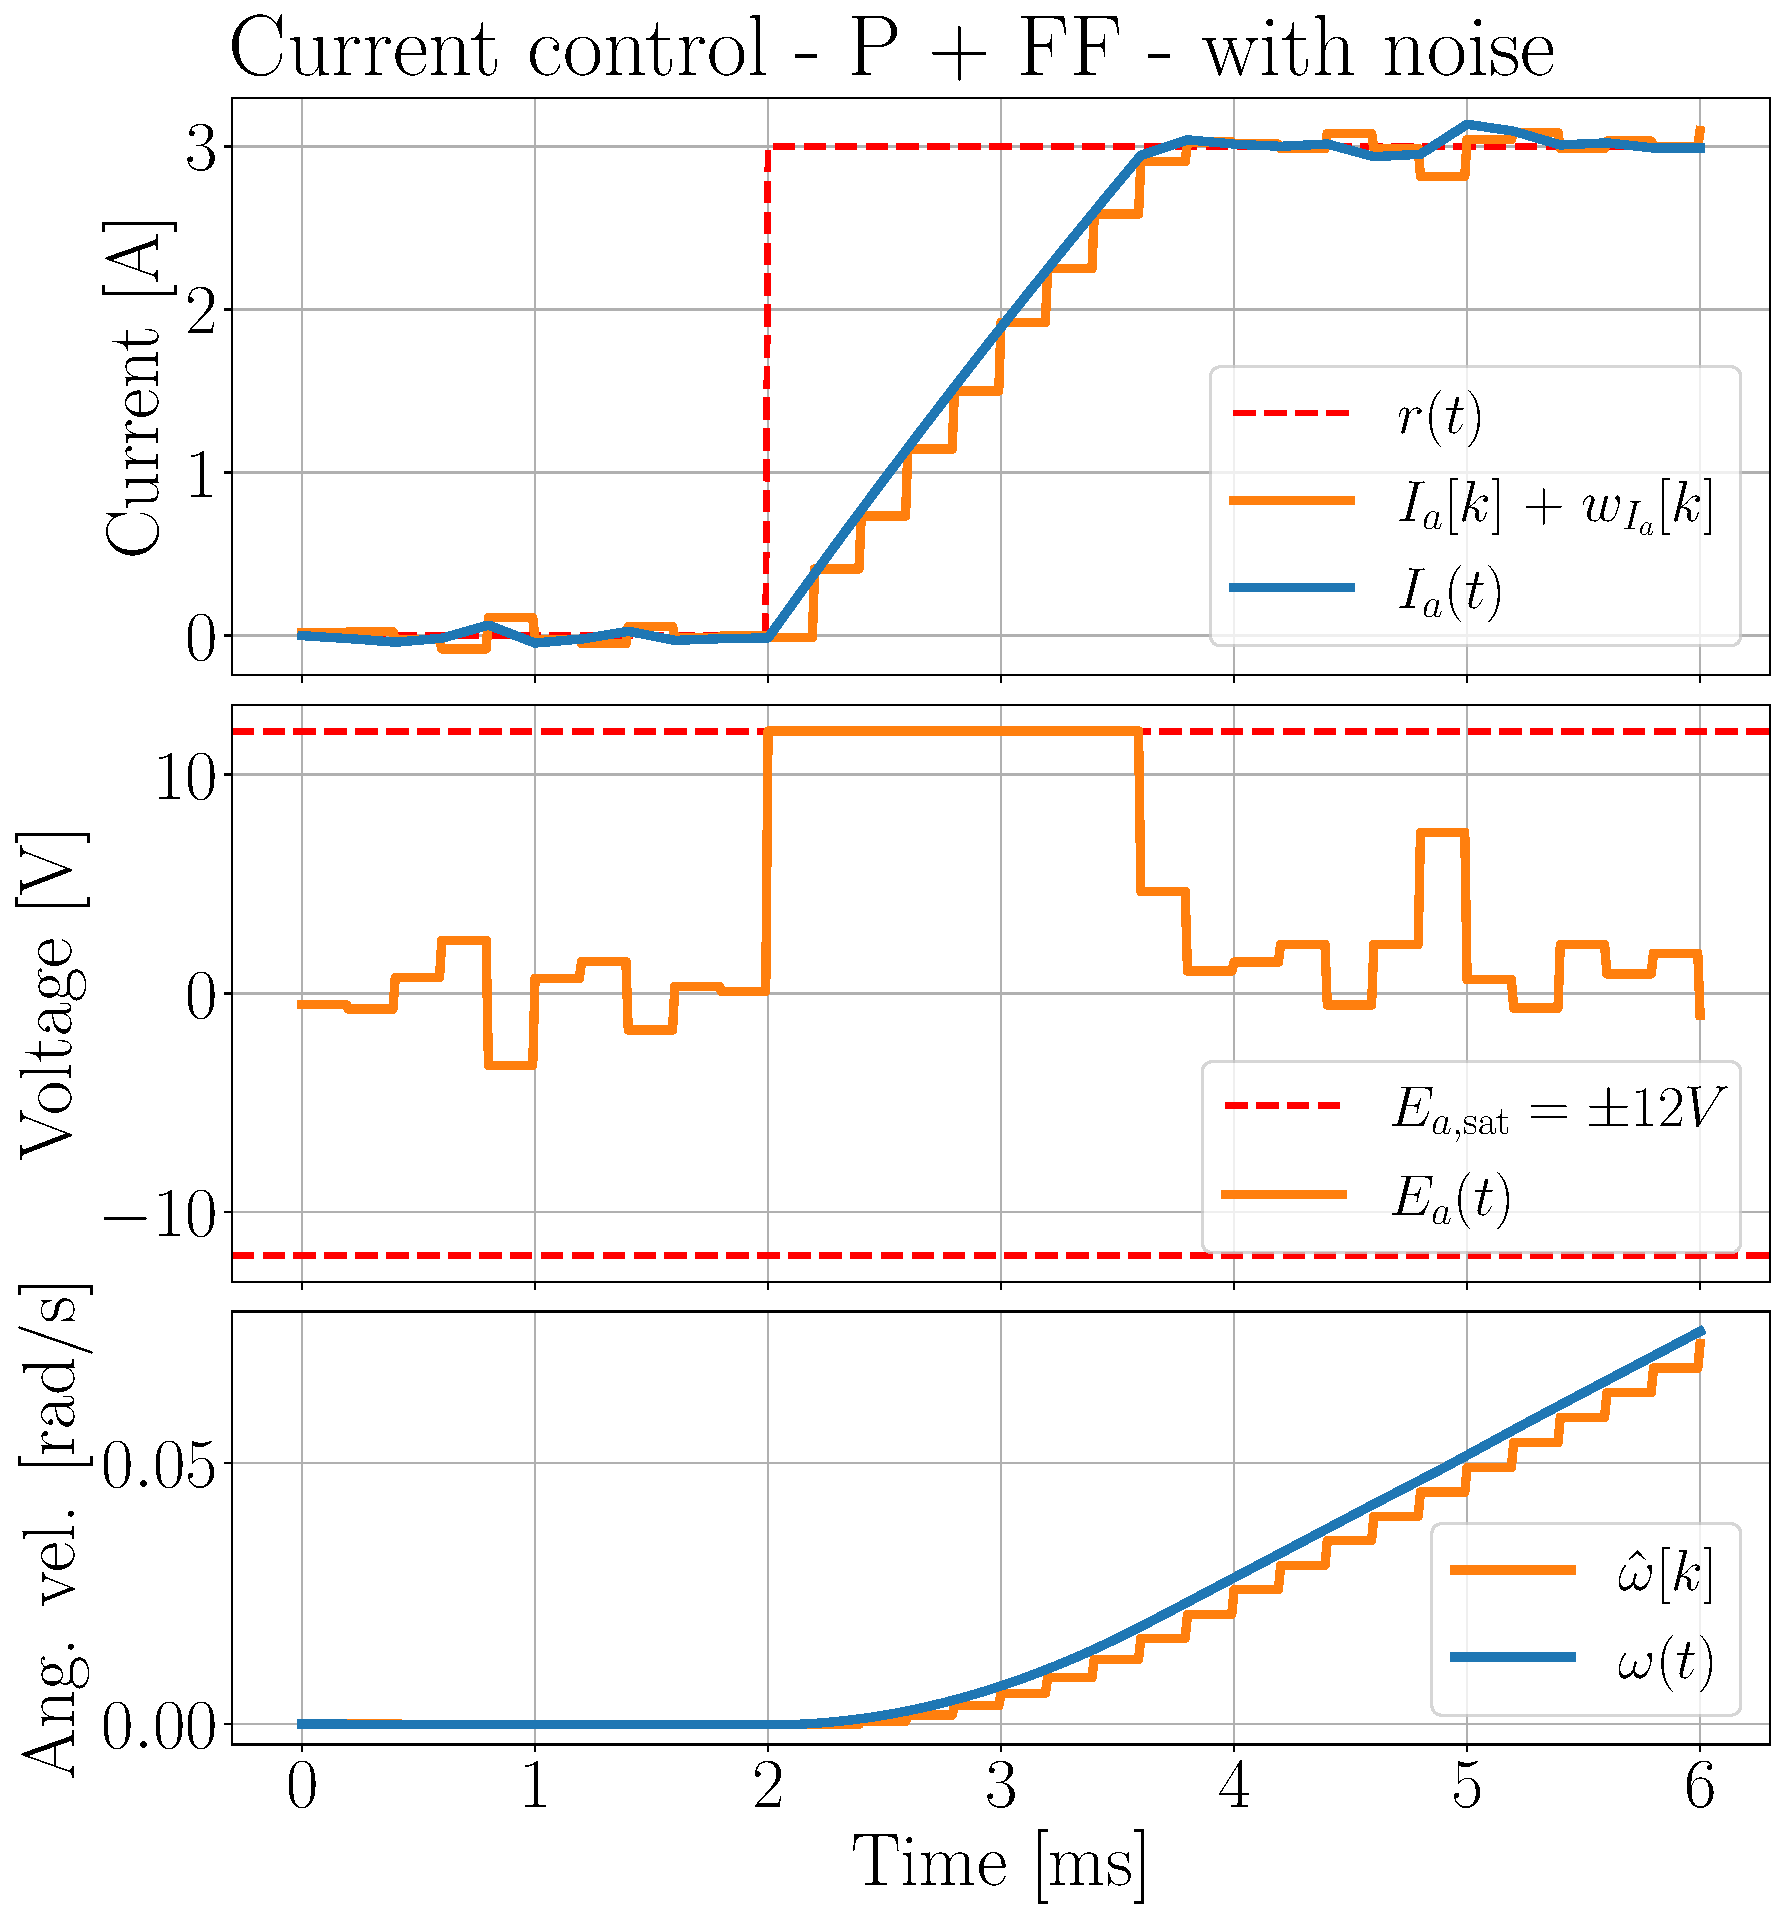
\includegraphics[width=0.49\textwidth]{../Figures/Controller_design/motor_current_control_feed_forward_P_FF_noise_Ts_0.2ms.pdf}}
    \caption{P+FF controller with and without noise, with $T_s = \SI{0.2}{\milli\second}$.}
    \label{fig:controller_design_current_controller_simulation_noise_0.2ms}
\end{figure}

\begin{figure}[htbp]
    \centering
    \subcaptionbox{Without noise.\label{fig:controller_design_current_controller_simulation_without_noise_1ms}}{%
        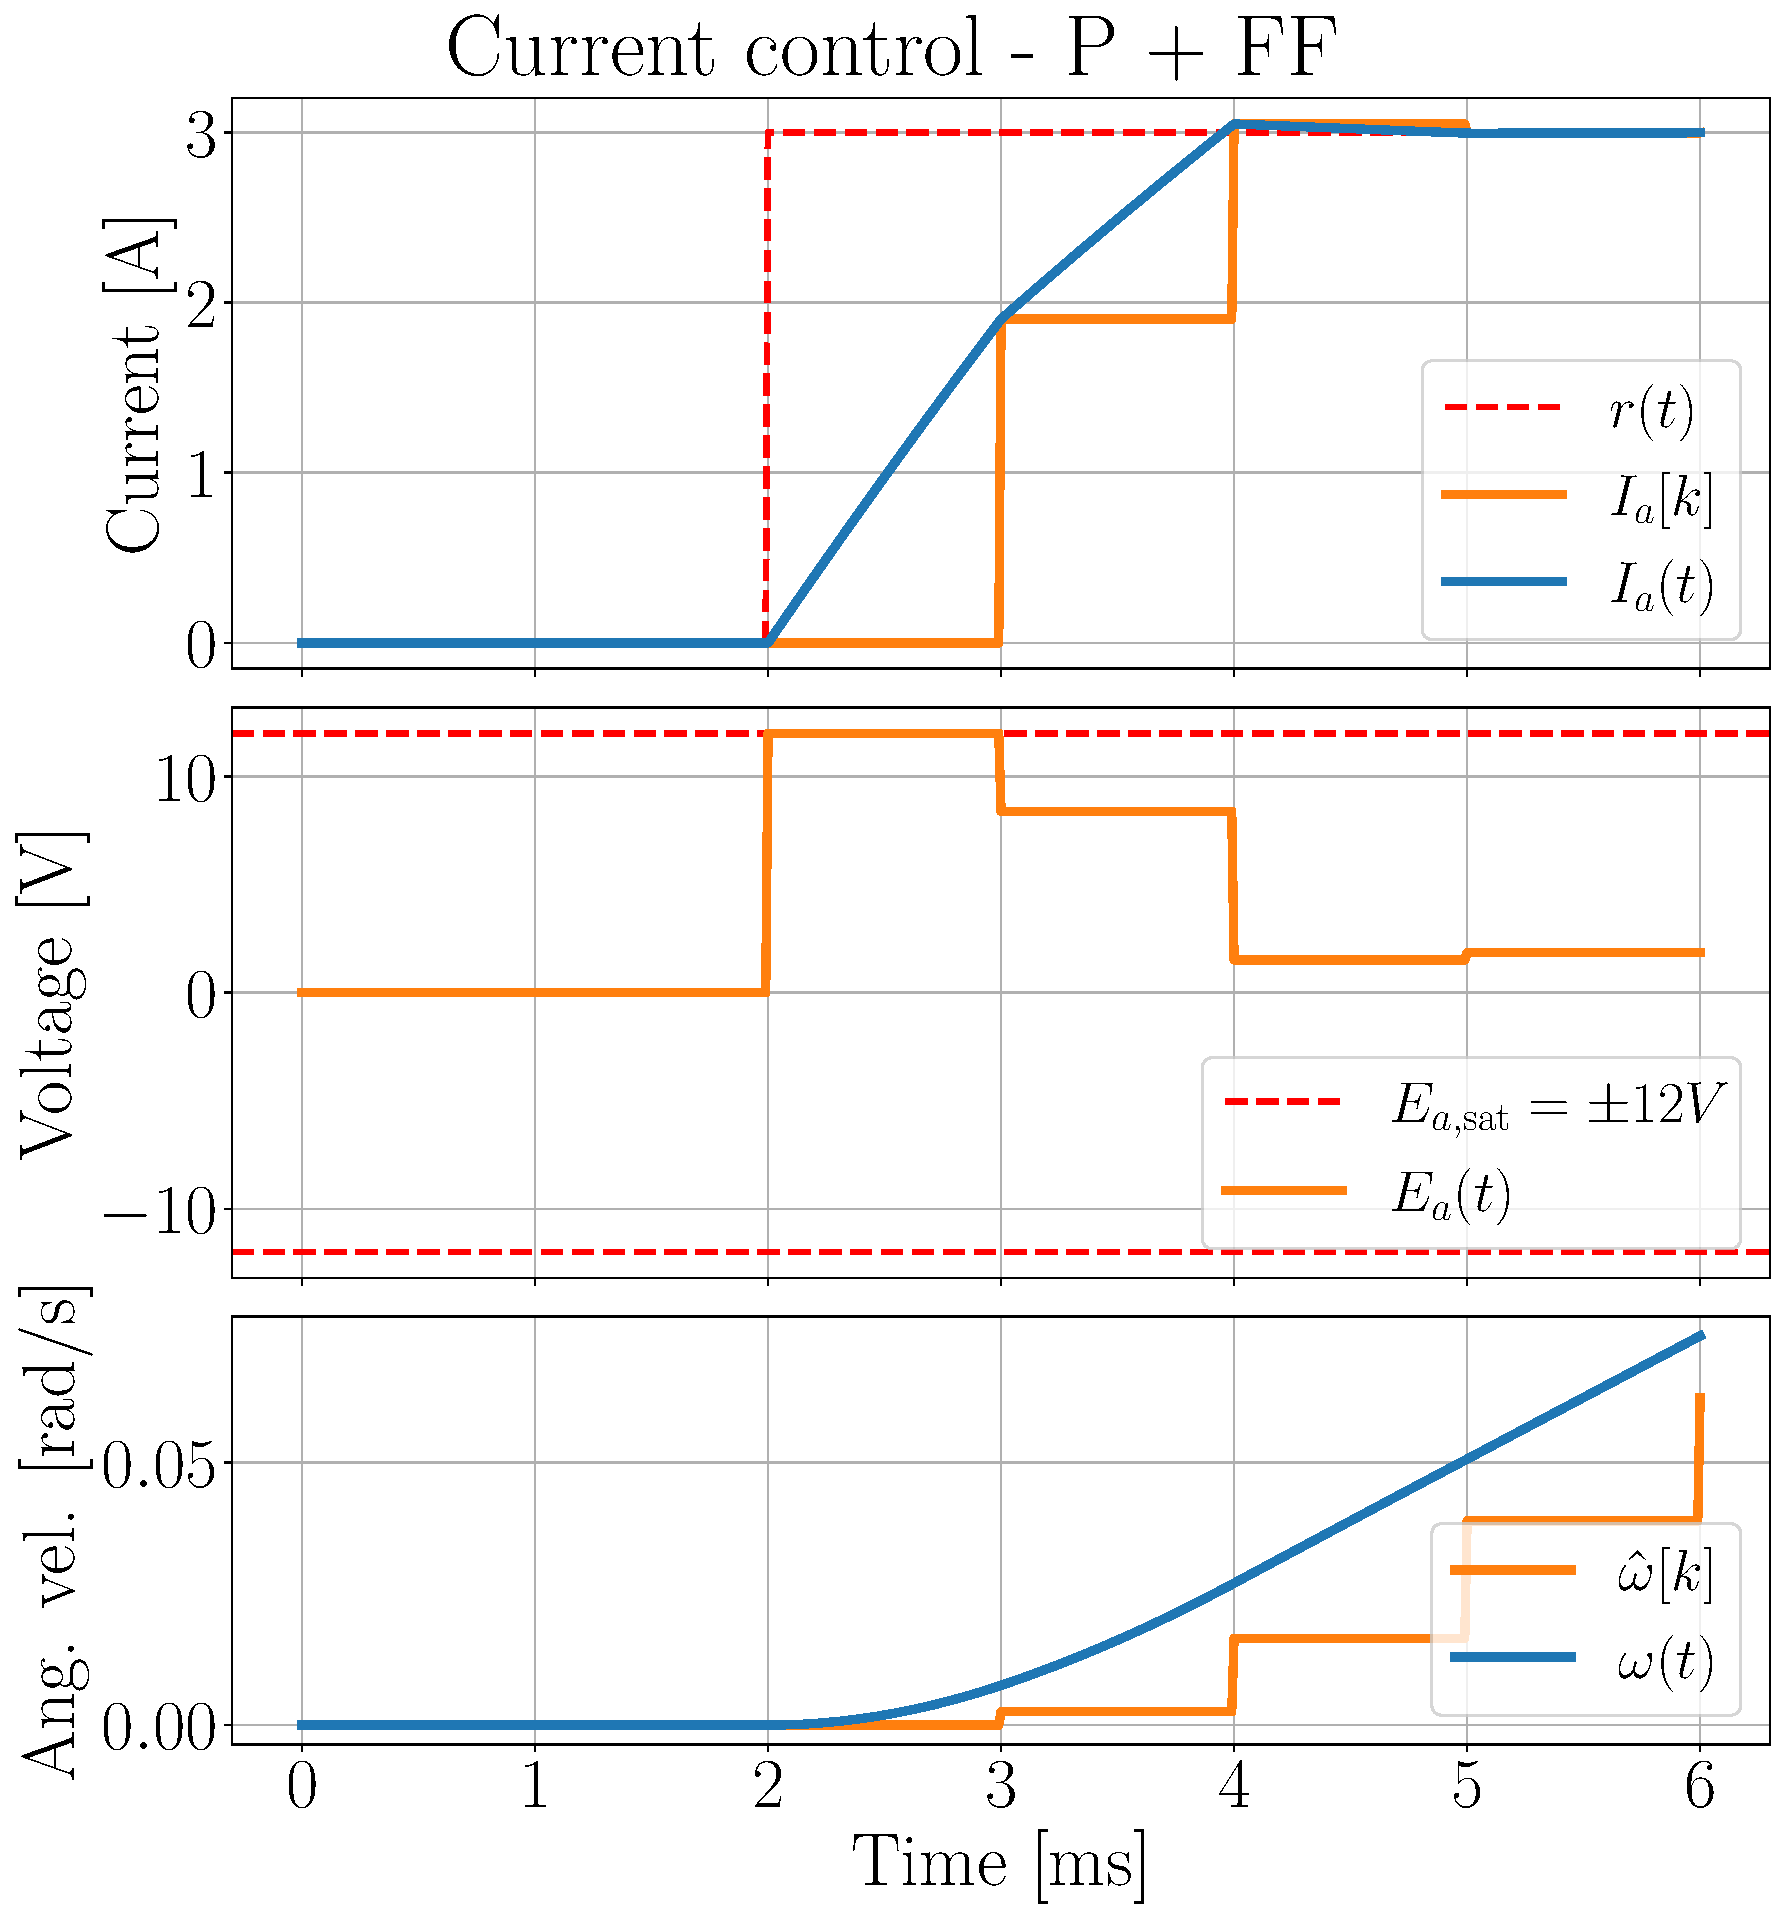
\includegraphics[width=0.49\textwidth]{../Figures/Controller_design/motor_current_control_feed_forward_P_FF_Ts_1.0ms.pdf}}
    \hfill
    \subcaptionbox{With noise.\label{fig:controller_design_current_controller_simulation_with_noise_1ms}}{%
        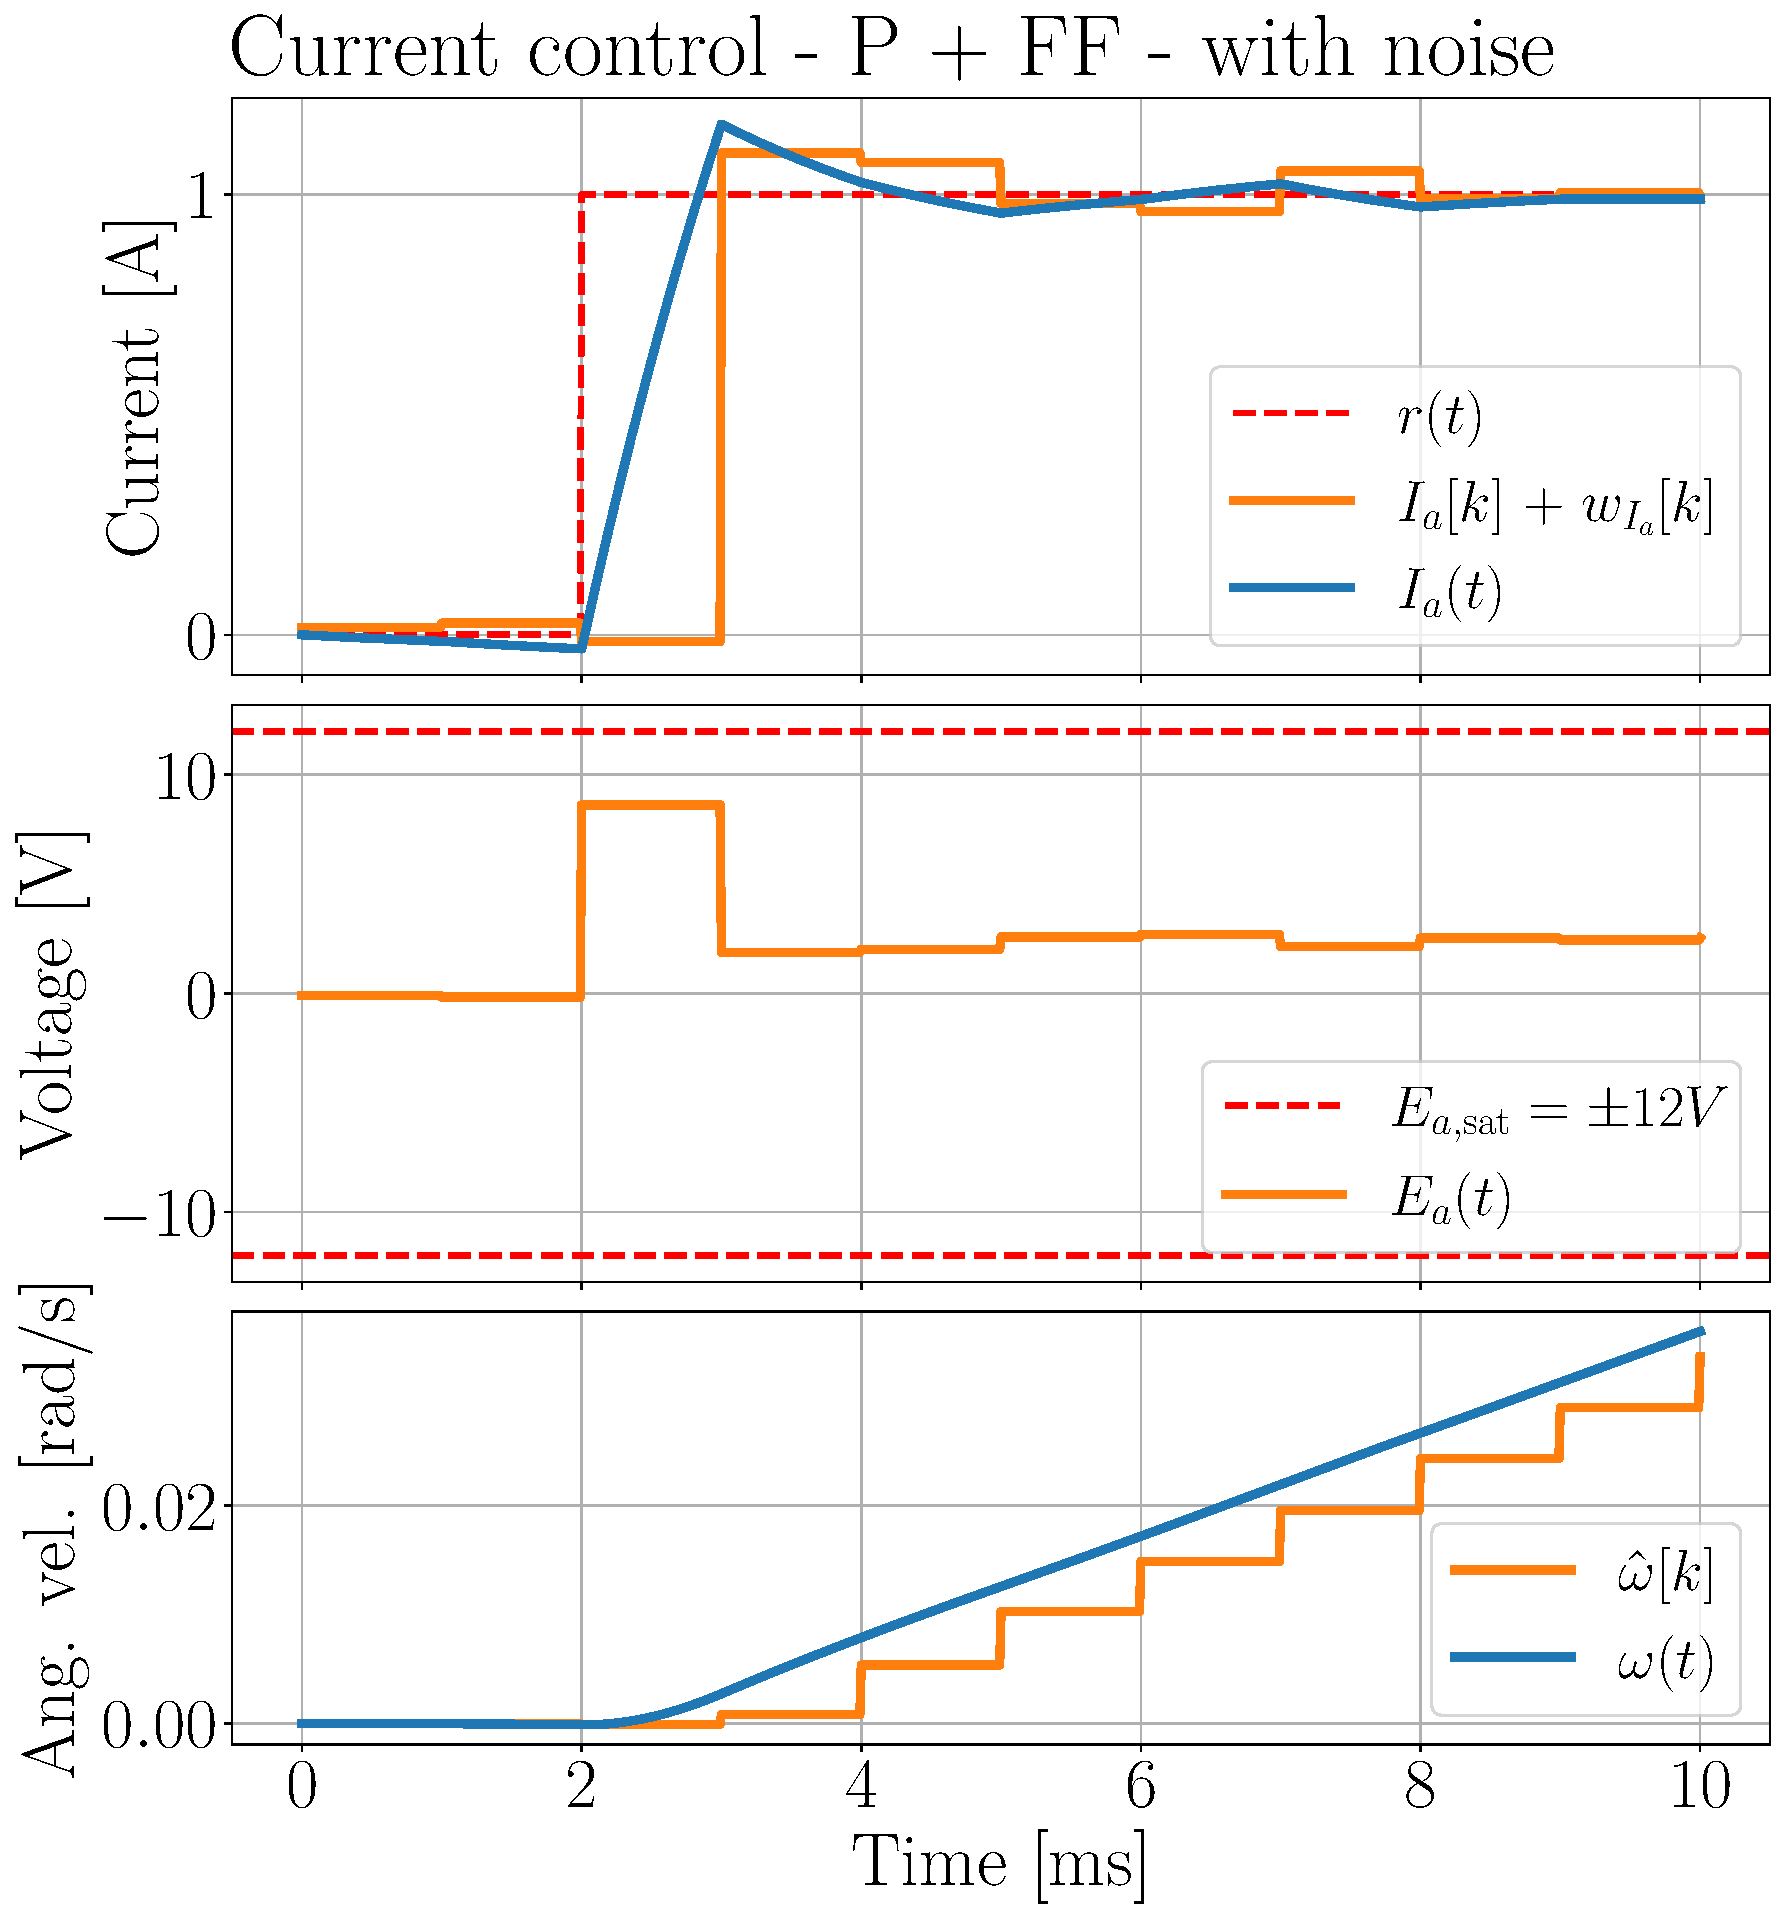
\includegraphics[width=0.49\textwidth]{../Figures/Controller_design/motor_current_control_feed_forward_P_FF_noise_Ts_1.0ms.pdf}}
    \caption{P+FF controller with and without noise, with $T_s = \SI{1.0}{\milli\second}$.}
    \label{fig:controller_design_current_controller_simulation_noise_1ms}
\end{figure}

\subsection{Evaluation of controller}

When the motor is starting from still, both the P+FF and P controllers are able to track the reference current well, as can be seen in \cref{fig:controller_design_current_controller_simulation_P_vs_PFF_no_speed}. However, when the motor is already spinning at a high speed, the P controller struggles to track the reference current and gets a steady-state error, as can be seen in \cref{fig:controller_design_current_controller_simulation_p_with_speed}. The P+FF controller on the other hand continues to perform well, as seen in \cref{fig:controller_design_current_controller_simulation_pff_with_speed}. This is because the back-EMF is significant at high speeds, and without the feedforward term, the P controller can't account for it. Realistically the motor won't be spinning at such high speeds most of the time. Therefore it might be tempting to remove the feedforward term. This could be a good idea for torque control, to simplify the controller, as described in [\textbf{ADD REFERENCE TO CONTROLLER DESIGN: TORQUE CONTROL}]. But for position control, I would advise against removing it, as the motor picks up speed in a relatively small amount of time. For robustness in general I would keep the feedforward term. 

\cref{fig:controller_design_current_controller_simulation_noise_1ms} and \cref{fig:controller_design_current_controller_simulation_noise_0.2ms} shows that the P+FF controller is able to track the reference current well with noise present in the current measurements, and even with a slower update period of $T_s = \SI{1.0}{\milli\second}$. The noise causes some jitter in the current, but it doesn't cause any significant issues for tracking the reference current.

Overall, the P+FF and P controllers show promising results for controlling the armature current in our system. Due to the saturation in the voltage of $E_a=\pm\SI{12}{\volt}$, there is a maximum rate of change for the current. During simulation it was found to be $\dot{I_a}_{\jnt{\text{max}}}\approx\SI{2.0}{\kilo\ampere\per\second}$, when the motor was starting from still, which is more or less instantaneous seen from the dynamics of the mechanical system. Hence, we will treat the armature current as a control input for further control design.

\section{Torque control}
\label{sec:controller_design_torque_control}

When the hand interracts with objects, trying to control the position of the hand becomes irrelevant, as the hand will be constrained by the object. Instead, we want to control the torque generated by the motor, which will allow us to control the force applied to the object.

As mentioned in \cref{sec:brushed_dc_motor_model}, the torque generated by the motor is proportional to the armature current:

\begin{equation}
    \label{eq:controller_design_torque_current_relation}
    \tau_m = K_t I_a.
\end{equation}

In \cref{sec:controller_design_current_controller}, we designed a controller for the armature current $I_a$ with the armature voltage $E_a$, and concluded that we can treat the armature current as a control input for further control design. Hence, we can directly control the torque by controlling the armature current. For a given reference torque $r_{\jnt{\tau_m}}$, we can calculate the reference current $r_{\jnt{I_a}}$ as:

\begin{equation}
    \label{eq:controller_design_torque_control_reference}
    r_{\jnt{I_a}} = \frac{r_{\jnt{\tau_m}}}{K_t}.
\end{equation}

When gripping an object, assuming the object is rigid and that the cable is inelastic, the angular velocity of the motor will be zero. Hence, the back-EMF will be zero. Therefore we can simplify the controller in \cref{eq:controller_design_voltage_input} to just a P controller. This will reduce the computational load on the microcontroller, and might get us better control over the torque.

\begin{figure}%
    \label{fig:controller_design_torque_control_rigid_object}
    \centering
    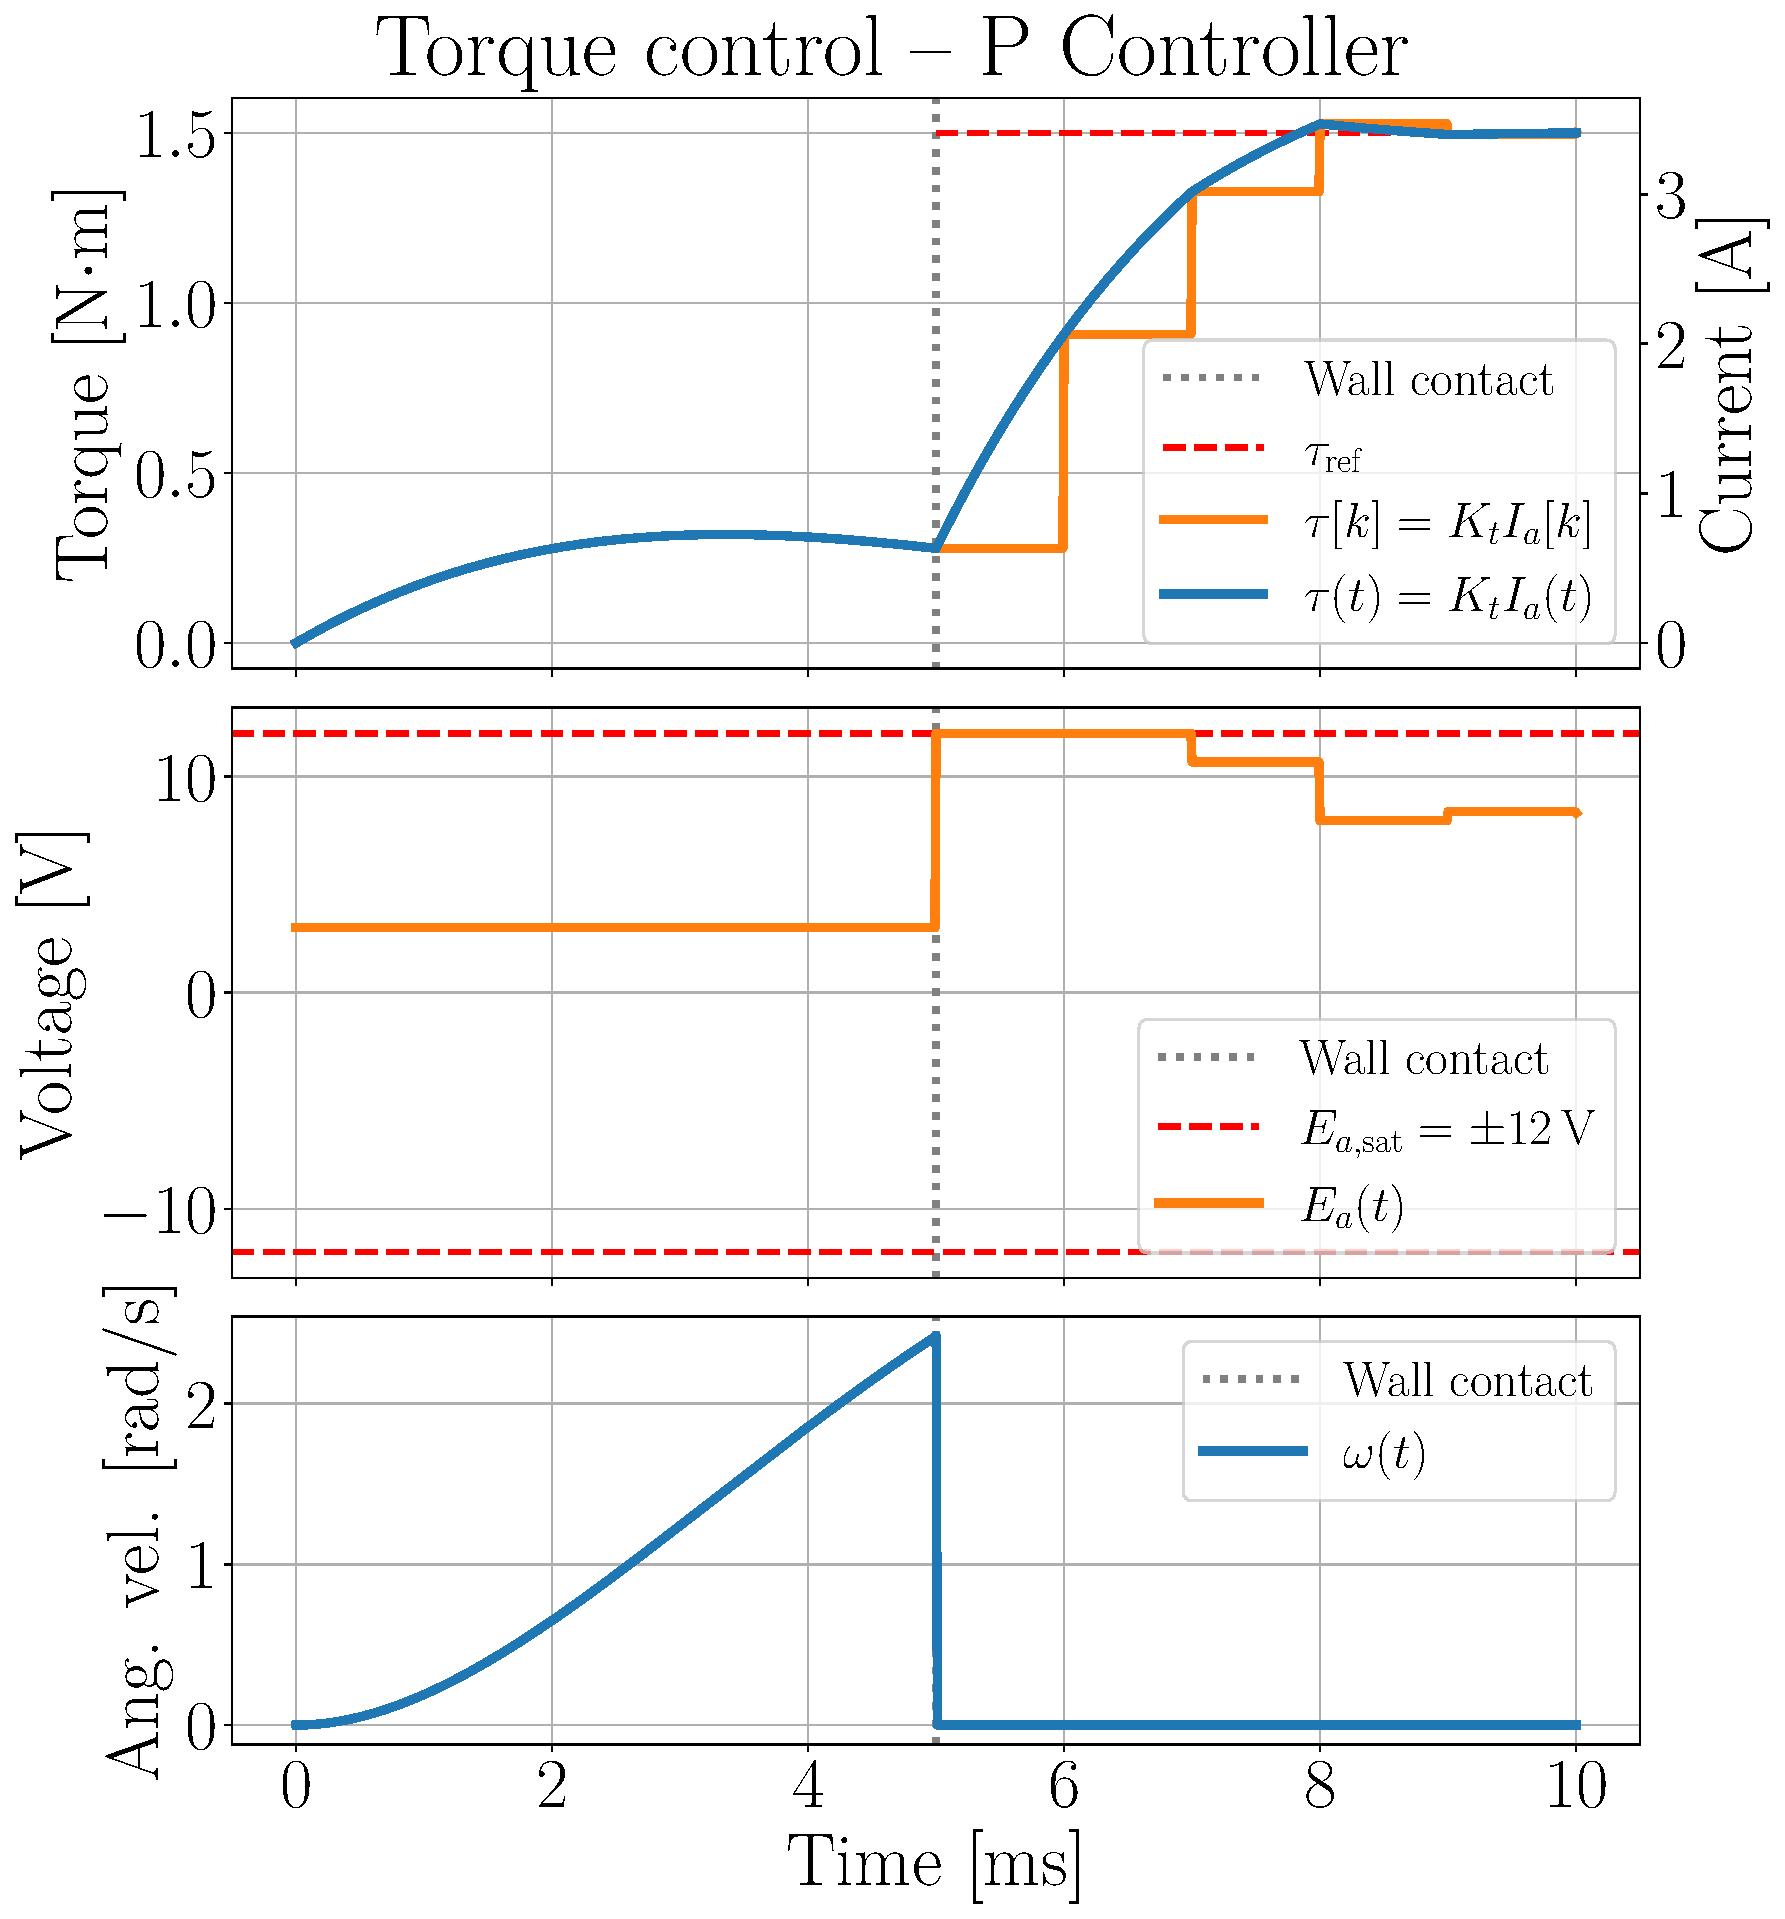
\includegraphics[width=0.8\textwidth]{../Figures/Controller_design/motor_torque_control_P_Ts_1.0ms.pdf}
    \caption{Torque control with a P controller when gripping a rigid object.}
\end{figure}

\section{Controllability of the system}%
\label{sec:controllability}
Based on the state-space representation our system in \cref{subsec:state_space_model_load}, we can check if the system is controllable, as described in \cref{subsec:theory_control_controllability}. The controllability matrix $\mathcal{C}$ for our system is given by:

\begin{equation}
    \label{eq:model_controllability}
    \mathcal{C} = [\mathbf{B}, \mathbf{A}\mathbf{B}, \mathbf{A}^2\mathbf{B}].
\end{equation}

Substituting for our specific $\mathbf{A}$ and $\mathbf{B}$, we get:

\begin{equation}
    \mathcal{C} = 
    \begin{bmatrix}
        0 & 0 & \frac{K_t}{L_a (J_m+J)}\\
        0 & \frac{K_t}{L_a (J_m+J)} & -\frac{K_t [L_a (B_m+c) + R_a (J_m+J)]}{L_a^2 (J_m+J)^2}\\
        \frac{1}{L_a} & -\frac{R_a}{L_a^2} & -\frac{K_b K_t L_a+R_a^2 (J_m+J)}{L_a^3 (J_m+J)}
    \end{bmatrix}.
\end{equation}

Clearly, $\mathrm{rank}(\mathcal{C}) = 3$, which is equal to the number of states. Therefore, the system is controllable.

\section{MRAC implementation}%
\label{sec:mrac_implementation}

